%!TEX program = xelatex
\PassOptionsToPackage{quiet}{xeCJK}
\documentclass[withoutpreface,bwprint]{cumcmthesis}
\usepackage{ctex}
\usepackage[numbers,sort&compress]{natbib}
\usepackage{amsmath,amssymb,bm}
\usepackage{booktabs,tabularx,multirow}
\usepackage{graphicx,float}
\usepackage{xcolor,url,listings}
\hypersetup{hidelinks}
\graphicspath{{../../../outputs/figures/}}
\setlist{nosep,leftmargin=2em}
\newcommand{\Rstar}{R^{*}}
\newcommand{\Pstar}{P^{*}}
\newcommand{\Ustar}{U^{*}}
\newcommand{\vect}[1]{\bm{#1}}
\definecolor{codeblue}{HTML}{24557A}
\definecolor{codegreen}{HTML}{3F6B4F}
\definecolor{codeorange}{HTML}{A15C20}
\definecolor{codegray}{HTML}{6B7280}
\lstset{
  basicstyle=\ttfamily\small,
  backgroundcolor=\color{gray!6},
  frame=single,
  framerule=0.4pt,
  rulecolor=\color{gray!35},
  xleftmargin=1em,
  xrightmargin=1em,
  aboveskip=0.6em,
  belowskip=0.8em,
  columns=fullflexible,
  keepspaces=true,
  showstringspaces=false
}
\lstdefinestyle{pythonappendix}{
  language=Python,
  basicstyle=\ttfamily\fontsize{7.4pt}{8.8pt}\selectfont,
  keywordstyle=\color{codeblue}\bfseries,
  commentstyle=\color{codegreen}\itshape,
  stringstyle=\color{codeorange},
  numberstyle=\ttfamily\tiny\color{codegray},
  numbers=left,
  numbersep=8pt,
  stepnumber=1,
  backgroundcolor=\color{gray!4},
  frame=single,
  framerule=0.45pt,
  rulecolor=\color{codeblue!45},
  framesep=5pt,
  xleftmargin=2.1em,
  xrightmargin=0.4em,
  framexleftmargin=1.5em,
  aboveskip=0.8em,
  belowskip=1.0em,
  columns=fullflexible,
  keepspaces=true,
  showstringspaces=false,
  breaklines=true,
  breakatwhitespace=false,
  breakindent=1.5em,
  postbreak=\mbox{\textcolor{codegray}{$\hookrightarrow$}\space},
  tabsize=4,
  captionpos=t
}
\renewcommand{\lstlistingname}{代码}
\renewcommand{\lstlistlistingname}{代码目录}
\title{芯片歧管式微通道热管理系统的建模与多目标优化}

\begin{document}
\pagenumbering{gobble}
\maketitle
\begin{abstract}
本文研究芯片歧管式微通道热管理系统，考察针肋宽度比 $\beta$、歧管深高比 $\eta$ 和针肋排数 $N$ 对无量纲热阻、压降和温度非均匀性的影响。赛题附件给出了结构参数、运行条件和 84 组数值结果。本文先分析系统内的流动与传热过程，再利用附件数据预测三项性能，进而进行多目标优化，并讨论指标权重变化和参数误差的影响。

问题一沿冷却液的实际流路分析歧管内的流量分配、微通道针肋换热以及芯片与衬底中的热传导，由此解释三个结构参数对压降和温度分布的影响。4 组无针肋数据表明，在附件参数范围内，压降随 $\eta$ 的变化近似符合 $\eta^{-2}$ 关系。加入 $N\beta^2$ 后，简化关系对全部 84 组数据的拟合达到 $R^2=0.9764$。

问题二将 4 组无针肋数据与 80 组有针肋数据分开处理，比较二次响应面、三次响应面和两种高斯过程模型。在按参数水平索引分散划分的五折交叉验证中，三次响应面对 $\Rstar$、$\Pstar$ 和 $\Ustar$ 的均方根误差（RMSE）分别为 $3.46\times10^{-7}$、$5.59\times10^{-4}$ 和 $3.00\times10^{-4}$。即使整体留出中央 20 组相邻参数组合，三项 RMSE 仍均不超过 $4.29\times10^{-4}$，故后续预测和优化采用三次响应面。

问题三逐一枚举 $N=2,3,\ldots,10$，在每个 $N$ 下搜索 $\beta$ 和 $\eta$，由此得到 Pareto 候选方案。三项指标归一化后，按最大偏差最小准则（Chebyshev 准则）求得 $\beta=0.22494$，工程上推荐 $\beta\approx0.225$、$\eta=4.50$、$N=6$。此时 $\Rstar$、$\Pstar$ 和 $\Ustar$ 分别为 0.73433、0.09800 和 0.79019。

问题四在权重三角形中改变三项指标的权重，计算各 Pareto 方案能够保持最优的权重区域。按主网格合并邻近设计后，推荐范围为 $0.215\leq\beta\leq0.224$、$\eta=4.5$、$N=3$--$4$，覆盖 51.66\% 的权重组合。固定这一区域后，仅保留附件中的偶数排数和加密连续参数网格所得覆盖率分别为 48.38\% 和 49.99\%。最后选取区域内单点权重范围最大的 $(0.224,4.50,4)$ 作为代表方案。

问题五比较两个推荐方案在 $\beta$ 和 $\eta$ 发生扰动时的性能变化，分别考察设计点附近的相对敏感度和给定误差区间内的最大增幅。当参数变化不超出附件范围且幅度不超过 $5\%$ 时，两种方案的总体最大增幅分别为 7.10\% 和 6.62\%，均由压降决定，热阻与温度非均匀性的增幅小于 0.7\%。按能量守恒估算，质量流量为额定值的 0.9 倍和 1.1 倍时，冷却液平均温升分别约为 9.56 K 和 7.83 K。该估算只反映冷却液温升，不用于计算三项无量纲指标。
\keywords{歧管式微通道；针肋；响应面模型；多目标优化；敏感性分析}
\end{abstract}

\pagenumbering{arabic}
\section{问题重述}
\subsection{问题背景}
Zhang 等（2023）在多核处理器热点管理研究中指出，局部热点不仅会抬高最高温度，还会影响器件可靠性\cite{Zhang2023}。随着芯片功率密度和集成度提高，散热设计既要降低整体温升，也要控制不同位置之间的温差。

微通道液冷依靠较大的固液接触面积强化换热，能够在有限空间内处理较高的热流密度，但细长通道也会带来较大的流动阻力。Sarangi 等（2014）研究的歧管式微通道将入口和出口歧管交替布置，把原本较长的微通道分成多个较短流动段。冷却液由入口歧管进入微通道，换热后再由出口歧管汇集\cite{Sarangi2014}。Wang（2011）的歧管流量分配理论和 Lee 等（2024）的一维模型均表明，歧管内的压力变化仍可能造成各微通道流量不均\cite{Wang2011,Lee2024}。针肋可以增加换热面积、扰动流体，却也会增加压力损失。选择结构参数时，散热能力、泵送代价和温度均匀性需要一并考虑。

\subsection{问题重述}
\begin{enumerate}[label=\textbf{（\arabic*）},leftmargin=3.2em]
  \item 建立结构参数、流量分配、微通道换热和温度分布之间的联系，解释三项性能指标的变化规律；
  \item 利用附件数据建立三项无量纲指标的预测模型，并检验模型的拟合效果和参数范围内的预测能力；
  \item 同时最小化热阻、压降和温度非均匀性，在没有额外指标权重信息时给出综合方案；
  \item 考察评价权重变化，寻找能适应多种指标权重的设计；
  \item 在假设的参数误差范围内比较代表方案，并讨论入口流量等运行条件发生变化时系统性能可能如何变化。
\end{enumerate}

\section{问题分析}
本题只给出了有限结构组合下的三个无量纲性能指标，无法据此还原各微通道内的流量、压力和温度。因此，问题一用简化的流动与传热关系解释三个结构参数的作用。问题二至问题五直接使用附件数据预测性能，随后讨论多目标优化、权重变化和参数误差。各部分之间的关系见图~\ref{fig:analysis-workflow}。
\subsection{问题一分析}
$\eta$ 会改变入口和出口歧管内的流速与压力分布，进而影响各微通道两端的压差。$\beta$ 和 $N$ 则主要影响针肋区的流动阻力与换热能力。歧管结构主要通过改变支路流量影响微通道换热。因此，问题一分别讨论歧管中的流量变化、微通道换热以及芯片和衬底中的导热，并用附件数据检验能够直接观察到的变化规律。

\subsection{问题二分析}
问题二的 80 组有针肋数据恰好落在规则参数网格上。若随机划分训练集和验证集，验证点附近通常仍有参数十分接近的训练样本，所得预测误差可能偏小。4 组无针肋数据又缺少相应的中间组合，不宜与其余样本共同拟合连续三变量模型。因此，预测模型只使用 $4\times4\times5$ 个有针肋组合，并采用五折交叉验证、留一交叉验证、整组留出部分 $N$ 水平、整体留出中央 20 组相邻参数四种方式检查预测误差。

\subsection{问题三分析}
三个单目标的最优结构并不一致，不存在一个在三项指标上同时最优的设计。由于 $N$ 只能取整数，而 $\beta$ 和 $\eta$ 可以连续变化，计算时对每个整数 $N$ 分别搜索 $\beta$ 和 $\eta$，汇总后筛选 Pareto 方案。三个指标的变化范围不同，需先按各自的理想值和 Pareto 前沿上的参考上界归一化，再从中选择最大归一化偏差最小的方案。

\subsection{问题四分析}
指标权重改变后，加权得分最小的设计也可能随之改变。三项非负权重之和为 1，可以用权重三角形表示。计算时先按固定步长离散 $\beta$ 和 $\eta$，再求各候选方案在权重三角形中的最优区域，同时比较单个网格点与邻近设计区域的结果。

\subsection{问题五分析}
参数误差只施加于连续参数 $\beta$、$\eta$，整数排数 $N$ 保持不变。尺寸变化很小时，可通过相对敏感度比较参数影响。误差达到几个百分点后，局部导数难以反映整个区间内的变化，因而还要分别计算各指标在给定误差区间内的最大增幅，并取三项最大增幅中的最大值作为总体指标。运行工况部分只用能量守恒估算质量流量变化后的冷却液平均温升，不据此预测三项无量纲指标。

\subsection{数据来源与使用边界}
本文所用原始数据均来自赛题材料。附件 1 给出结构尺寸、材料参数和运行条件，附件 2 给出 84 组结构组合及对应的 $\Rstar$、$\Pstar$、$\Ustar$，其中 4 组无针肋、80 组有针肋。附件未给出三个指标的具体无量纲化定义，问题一因此只分析它们对应的物理量及变化趋势。自问题二起，预测和优化直接使用附件给出的三个无量纲数值。下文未特别说明时，“附件数据”均指附件 2。

\begin{figure}[H]
\centering
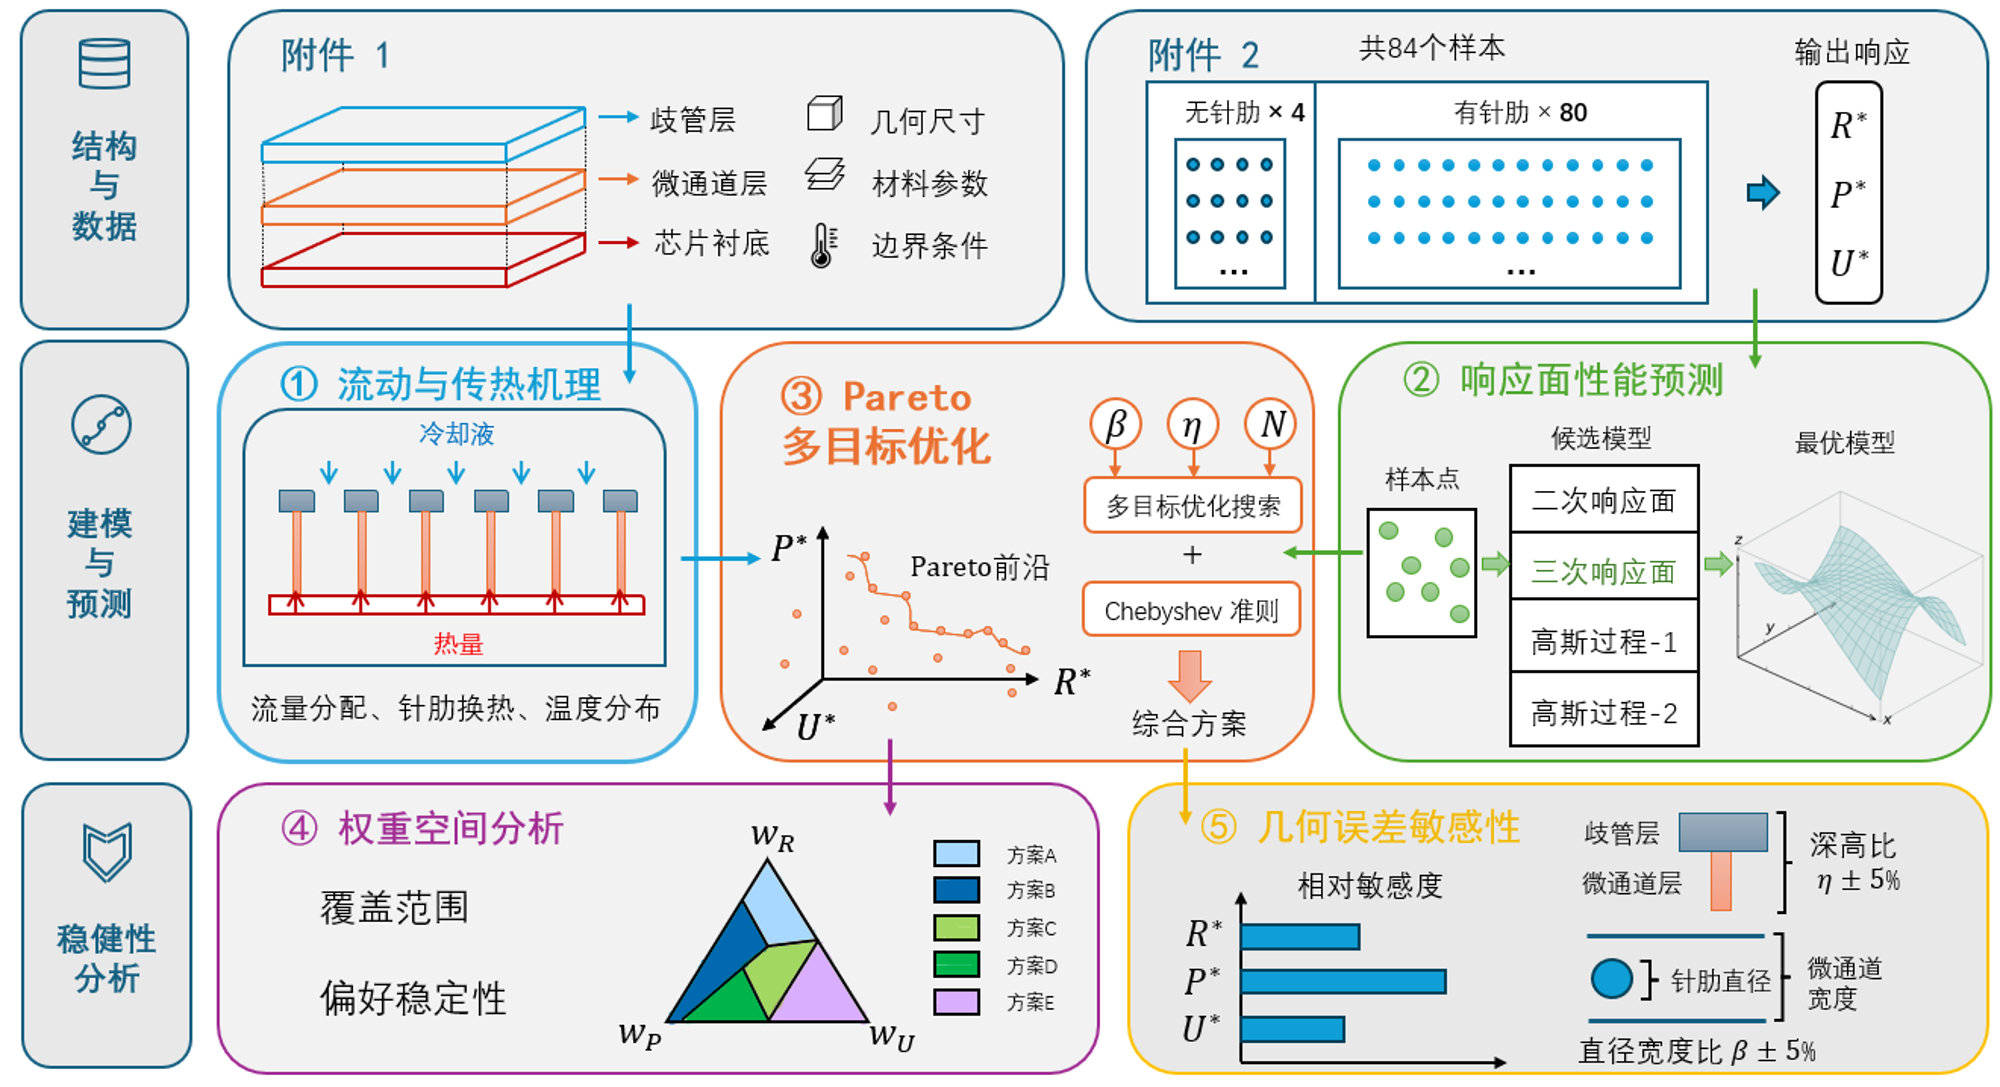
\includegraphics[width=0.98\textwidth]{fig_analysis_workflow.png}
\caption{全文分析流程。附件 1 用于确定系统结构、材料参数和运行条件，附件 2 用于检验问题一中的变化规律，并建立后续的性能预测和优化模型。}
\label{fig:analysis-workflow}
\end{figure}

\section{模型假设}
为简化模型，本文作如下假设：
\begin{enumerate}[label=\arabic*.,leftmargin=2.5em]
  \item 冷却液作稳态、单相、不可压缩流动，材料物性在附件给定温度附近取常数；
  \item 芯片体积热源在中央 $6\,\mathrm{mm}\times6\,\mathrm{mm}$ 区域内均匀分布；
  \item 为分析歧管中的流量分配，只取一组相邻的入口歧管、出口歧管及两者之间的微通道建立简化模型。该模型不再逐一描述三个入口和两个出口之间的整体差异，所得变化规律由附件给出的总体性能数据检验；
  \item 芯片和衬底的厚度远小于平面尺寸，因此用厚度方向的平均温度描述平面内温度变化，不再逐层求解厚度方向的温度分布。平面内导热用 $K_{\parallel}$ 表示，固体与冷却液之间的换热用 $g(x,y)$ 表示；
  \item 根据第~5.2 节的量级估计，辐射及外表面自然对流相对液冷散热为小量，在主模型中忽略。
\end{enumerate}

\section{符号说明}
\begin{table}[H]
\centering
\caption{主要符号、含义及单位}
\small
\setlength{\tabcolsep}{4pt}
\begin{tabularx}{\textwidth}{cXc cXc}
\toprule
符号 & 含义 & 单位 & 符号 & 含义 & 单位\\
\midrule
$\beta$ & 针肋直径与微通道宽度之比 & -- & $\eta$ & 歧管层与微通道层的深高比 & --\\
$N$ & 沿微通道流向的针肋排数 & -- & $q_i$ & 第 $i$ 个微通道支路的体积流量 & $\mathrm{m^3\,s^{-1}}$\\
$\mathcal Q_i^{\mathrm{in}},\mathcal Q_i^{\mathrm{out}}$ & 第 $i$ 个位置处入口歧管剩余流量、出口歧管已汇集流量 & $\mathrm{m^3\,s^{-1}}$ & $\mathcal Q_{\mathrm{tot}},\mathcal Q_g$ & 系统总体积流量、分配给所取支路组的入口流量 & $\mathrm{m^3\,s^{-1}}$\\
$P_i^{\mathrm{in}},P_i^{\mathrm{out}}$ & 对应轴向位置入口、出口歧管的压力 & $\mathrm{Pa}$ & $\Delta P_i$ & 第 $i$ 个微通道支路两端的压差 & $\mathrm{Pa}$\\
$R_d$ & 平均流量处压差随流量变化的斜率 & $\mathrm{Pa\,s\,m^{-3}}$ & $G_i$ & $h_iA_{\mathrm{eff},i}$，即传热率与固液温差之比 & $\mathrm{W\,K^{-1}}$\\
$G_0$ & 平均支路流量下的 $G_i$ & $\mathrm{W\,K^{-1}}$ & $\mathcal Q_{m,r}$ & 进入第 $r$ 个完整入口歧管的流量 & $\mathrm{m^3\,s^{-1}}$\\
$\bar q$ & 当前支路组的平均支路流量 & $\mathrm{m^3\,s^{-1}}$ & $g(x,y)$ & 单位面积上，传热率与固液温差之比 & $\mathrm{W\,m^{-2}K^{-1}}$\\
$T_s,T_f$ & 固体温度、冷却液代表温度 & $\mathrm{K}$ & $\dot Q_{f,i}$ & 冷却液带走的传热率 & $\mathrm{W}$\\
$K_{\parallel}$ & 厚度积分后的面内导热参数 & $\mathrm{W\,K^{-1}}$ & $\psi$ & 支路流量变化对 $G_i$ 影响的无量纲函数 & --\\
$\vect x$ & 编码后的设计变量 & -- & $\Rstar$ & 无量纲热阻 & --\\
$\Pstar$ & 无量纲压降 & -- & $\Ustar$ & 无量纲温度非均匀性 & --\\
$S_{jk}$ & 相对敏感度 & -- & $\vect f^I,\vect f^{\mathrm{ref}}$ & 理想值、归一化参考上界 & --\\
$\vect w$ & 三项指标的非负权重 & -- & $B_i$ & 方案 $i$ 成为最优时对应的权重范围占比 & --\\
$\vect f$ & 三项性能指标组成的向量 & -- & $p_k$ & 敏感度分析中的连续参数 & --\\
\bottomrule
\end{tabularx}
\end{table}

\begin{table}[H]
\centering
\caption{主要物理常数、材料参数与运行条件}
\label{tab:physical-parameters}
\small
\begin{tabular}{llrlc}
\toprule
参数 & 符号 & 数值 & 单位 & 来源\\
\midrule
水的密度 & $\rho$ & 998.2 & $\mathrm{kg\,m^{-3}}$ & 附件 1\\
水的定压比热容 & $c_p$ & 4182 & $\mathrm{J\,kg^{-1}K^{-1}}$ & 附件 1\\
水的导热系数 & $k_f$ & 0.6 & $\mathrm{W\,m^{-1}K^{-1}}$ & 附件 1\\
水的动力黏度 & $\mu$ & 0.001003 & $\mathrm{Pa\,s}$ & 附件 1\\
氮化铝导热系数 & $k_{\mathrm{AlN}}$ & 200 & $\mathrm{W\,m^{-1}K^{-1}}$ & 附件 1\\
芯片等效导热系数 & $k_{\mathrm{chip}}$ & 298 & $\mathrm{W\,m^{-1}K^{-1}}$ & 附件 1\\
芯片厚度 & $t_{\mathrm{chip}}$ & 200 & $\mu\mathrm{m}$ & 附件 1\\
芯片体积发热率 & $q'''$ & $5\times10^9$ & $\mathrm{W\,m^{-3}}$ & 附件 1\\
入口质量流量 & $\dot m_{\mathrm{in}}$ & 1 & $\mathrm{g\,s^{-1}}$ & 附件 1\\
入口温度 & $T_{\mathrm{in}}$ & 293 & $\mathrm K$ & 附件 1\\
外表面对流换热系数 & $h_{\mathrm{amb}}$ & 10 & $\mathrm{W\,m^{-2}K^{-1}}$ & 附件 1\\
\bottomrule
\end{tabular}
\end{table}

\section{问题一：流动与传热模型}
\subsection{系统结构与参数}
\subsubsection{系统结构与工作过程}
赛题附件 1 所示冷却结构的平面尺寸为 $10\,\mathrm{mm}\times10\,\mathrm{mm}$，中央 $6\,\mathrm{mm}\times6\,\mathrm{mm}$ 区域为芯片热源。歧管层由交替排列的入口流道和出口流道组成，下方是带圆柱针肋的微通道层。冷却液从顶部进入入口歧管，向下流入微通道，在针肋之间横向流动并吸收热量，随后向上进入相邻的出口歧管，最后从侧部排出。Sarangi 等（2014）和 Lee 等（2024）的歧管微通道模型也采用了这种包含多次近似 $90^\circ$ 转向的流动方式\cite{Sarangi2014,Lee2024}。入口和出口歧管的交替布置把较长的微通道分成了多个较短换热段。

歧管和微通道位于不同高度。入口流道将低温冷却液送往各微通道，出口流道则收集已经吸热的冷却液，两者通过下方的微通道相连。各微通道的流量取决于其两端所连接的入口歧管与出口歧管之间的压力差。图~\ref{fig:system-structure} 分别从整体结构、俯视和剖面三个角度说明这一流动过程。

\begin{figure}[H]
\centering
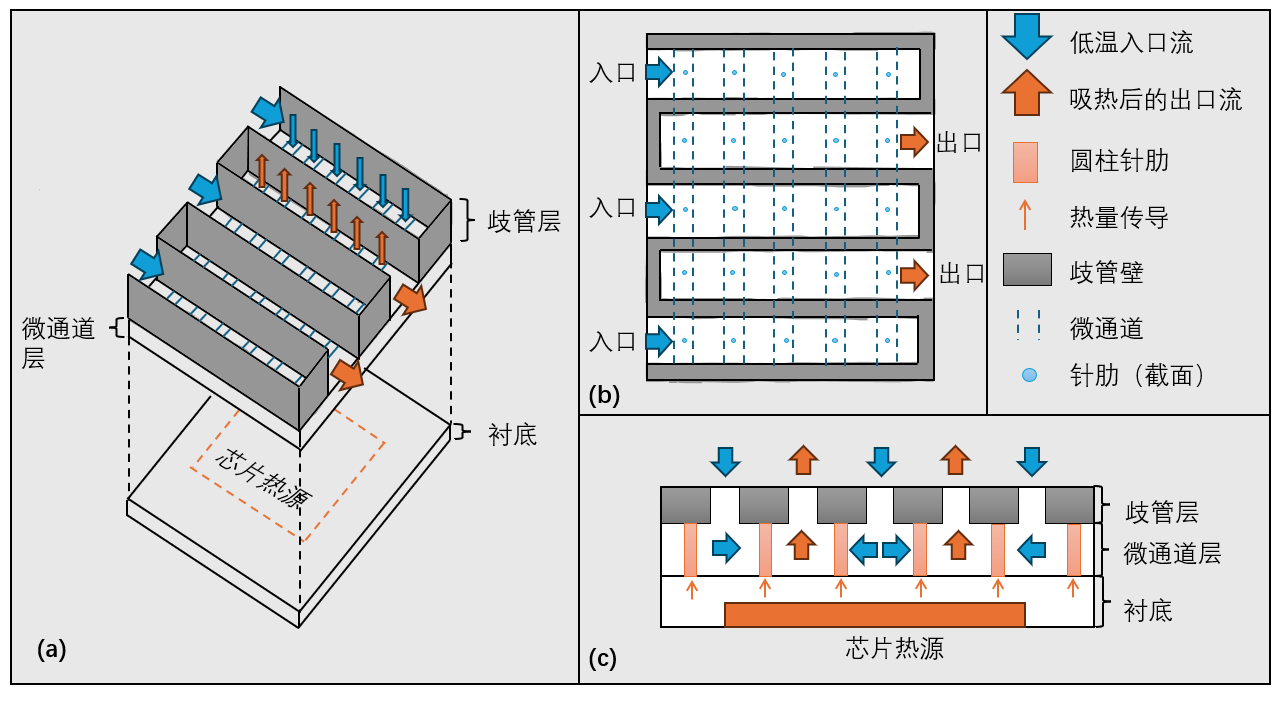
\includegraphics[width=0.98\textwidth]{fig_system_structure.png}
\caption{歧管式微通道热管理系统的结构与冷却液流动路径。（a）歧管、微通道、衬底和芯片热源的整体关系；（b）入口歧管、出口歧管与微通道的俯视关系；（c）冷却液从入口歧管进入针肋微通道、吸热后再进入出口歧管的剖面示意。蓝色表示低温冷却液，橙色表示吸热后的冷却液，细橙色箭头表示热量传递。为同时展示流动和传热路径，子图（a）、（c）沿厚度方向翻转绘制，图中尺寸不按比例。}
\label{fig:system-structure}
\end{figure}

微通道能够在较小体积内提供较大的固液接触面积，局部换热可写为 $\dot Q=hA(T_w-T_f)$，其中 $h$ 为对流换热系数，$A$ 为有效换热面积，$T_w$ 为壁面温度。增大 $A$ 或 $h$ 有利于降低壁面与冷却液之间的温差，但通流空间减小也会增加阻力。Pan 等（2022）和 Jung 等（2021）的研究表明，圆柱针肋既能增加换热表面积并扰动速度边界层和热边界层，也会因绕流和局部收缩带来额外压力损失\cite{Pan2022,Jung2021}。Pan 等（2024）开展的实验进一步显示，针肋歧管微通道的流动和换热性能会随入口流量明显变化\cite{Pan2024Experimental}。

\subsubsection{关键结构参数}
针肋宽度比 $\beta=d_p/w_c$ 是针肋直径 $d_p$ 与微通道宽度 $w_c$ 之比。增大 $\beta$ 通常会增加换热面积并加强对流体的扰动，但留给冷却液的通流空间也会缩小。歧管深高比 $\eta=H_m/H_c$ 是歧管高度 $H_m$ 与微通道高度 $H_c$ 之比。总流量不变时，$\eta$ 越大，歧管截面积越大，平均流速越低。针肋排数 $N$ 按微通道流动方向计数，该方向与歧管中的主流方向不同。增加排数可以扩大换热面积、增强扰动，但后排针肋会受到前排尾流影响，综合性能未必随 $N$ 持续改善。Vilarrubí 等（2018）的研究表明，针肋沿程布置会影响温度均匀性\cite{Vilarrubi2018}。本题中冷却液还会沿程升温，使不同位置的针肋处在不同换热条件下。三个参数都会影响流量和换热，不能把其中某个参数只与一项性能指标对应。

\subsubsection{参数如何影响性能}
结构参数并不直接决定三项总体指标，其影响要经过支路压差与流量、局部换热和冷却液升温，最后反映在芯片和衬底的温度分布上：
\begin{equation}
(\beta,\eta,N)\rightarrow\{P_i^{\mathrm{in}}-P_i^{\mathrm{out}},q_i\}
\rightarrow\{G_i,T_{f,i}\}\rightarrow T_s(x,y)
\rightarrow\{\text{总体热阻},\Delta P,\text{温度非均匀性}\}.
\label{eq:causal}
\end{equation}
其中，$\eta$ 主要影响歧管中的压力分布，$\beta$ 和 $N$ 主要影响微通道内的阻力与换热，支路流量 $q_i$ 把两者联系起来。下文按式~\eqref{eq:causal} 中各环节的先后关系展开。

\subsection{基本热量估算}
赛题附件 1 给出芯片厚度 $200\,\mu\mathrm{m}$ 和体积发热率 $5\times10^9\,\mathrm{W\,m^{-3}}$，相应总发热量为
\begin{equation}
\dot Q_{\mathrm{chip}}=5\times10^9\times6\times10^{-3}\times6\times10^{-3}
\times200\times10^{-6}=36\ \mathrm W.
\end{equation}
在后面的二维导热方程中，将体积热源沿芯片厚度积分，得到面热源
\begin{equation}
q''_{\mathrm{gen}}(x,y)=
\begin{cases}
q'''t_{\mathrm{chip}}=10^6\ \mathrm{W\,m^{-2}}, & (x,y)\in\Omega_{\mathrm{chip}},\\
0, & (x,y)\notin\Omega_{\mathrm{chip}}.
\end{cases}
\label{eq:source}
\end{equation}
即面热源只作用在中央 $6\,\mathrm{mm}\times6\,\mathrm{mm}$ 的芯片区域，并未平均铺到整个散热面上。

附件 1 还给出入口温度 $293\,\mathrm K$、入口质量流量 $1\,\mathrm{g\,s^{-1}}$、氮化铝导热系数 $200\,\mathrm{W\,m^{-1}K^{-1}}$ 和芯片等效材料导热系数 $298\,\mathrm{W\,m^{-1}K^{-1}}$。若暂不计其他散热途径，把 $36\,\mathrm W$ 热量全部视为由冷却液带走，取附件中的 $c_p=4182\,\mathrm{J\,kg^{-1}K^{-1}}$，冷却液平均温升为
\begin{equation}
\Delta\bar T_f=\frac{36}{0.001\times4182}=8.61\ \mathrm K.
\label{eq:coolant-rise}
\end{equation}
$8.61\,\mathrm K$ 的温升表明，冷却液沿程升温不能忽略。外表面换热面积按 $10^{-4}\,\mathrm{m^2}$ 估计，自然对流系数取 $10\,\mathrm{W\,m^{-2}K^{-1}}$。即使表面与环境相差 $50\,\mathrm K$，自然对流散热也只有约 $0.05\,\mathrm W$。辐射散热也按 $50\,\mathrm K$ 温差估算，取表面温度 $T_s=343\,\mathrm K$、环境温度 $T_\infty=293\,\mathrm K$，并令表面发射率 $\varepsilon=1$。由 Stefan--Boltzmann 定律，
\begin{equation}
\dot Q_{\mathrm{rad}}=\varepsilon\sigma A(T_s^4-T_\infty^4)\approx0.037\ \mathrm W.
\end{equation}
其中 $\sigma=5.67\times10^{-8}\,\mathrm{W\,m^{-2}K^{-4}}$ 为 Stefan--Boltzmann 常数。
两者都只有芯片发热量的千分之一量级，因此主模型忽略外表面自然对流和辐射。

\subsection{模型建立}
以下分别建立歧管内的流量与压力关系、单条微通道内的换热关系，以及芯片和衬底中的二维导热方程。附件缺少局部流道尺寸、损失系数和各支路压力，因而这些方程只用于说明内部变量之间的关系，不能据此求出各支路流量和完整温度场。前述关系中可由附件数据直接检验的部分将在第~5.4 节讨论。

\subsubsection{歧管中的流量与压降}
为描述歧管中的流量变化，取图~\ref{fig:system-structure} 中一组由入口歧管连向相邻出口歧管的微通道支路，沿所取支路组从入口侧向出口汇集侧依次编号为 $i=1,\ldots,M$。记 $\mathcal Q_i^{\mathrm{in}}$ 为流到第 $i$ 个位置前、分配给这组支路且尚未分出的体积流量，$\mathcal Q_i^{\mathrm{out}}$ 为相邻出口歧管在该位置前已经汇集的体积流量，$q_i$ 为第 $i$ 个微通道的流量。

\begin{figure}[H]
\centering
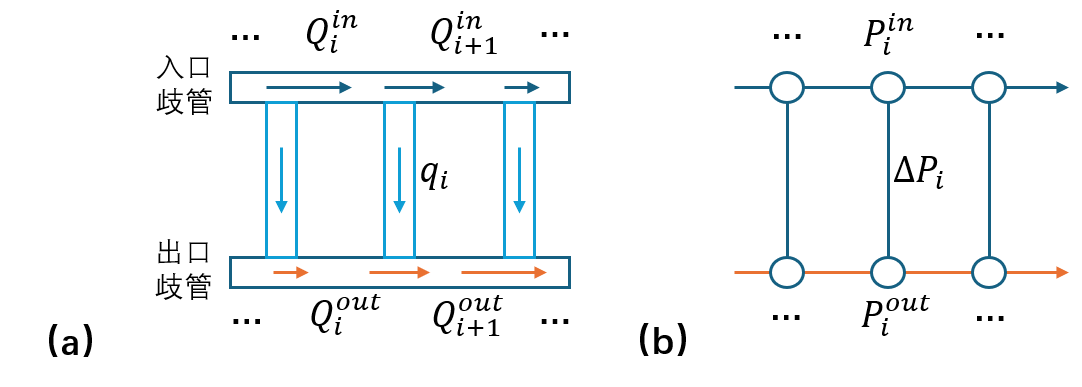
\includegraphics[width=0.90\textwidth]{fig_q1_hydraulic.png}
\caption{歧管与微通道支路的流量和压力关系。（a）入口歧管沿程向各微通道分流，出口歧管沿程汇集各支路流量，$\mathcal Q_i^{\mathrm{in}}$ 和 $\mathcal Q_i^{\mathrm{out}}$ 分别表示第 $i$ 个位置前的入口歧管剩余流量和出口歧管已汇集流量，$q_i$ 为第 $i$ 个支路流量；（b）对应位置的入口、出口歧管压力及支路压差 $\Delta P_i=P_i^{\mathrm{in}}-P_i^{\mathrm{out}}$。水平箭头表示歧管内主流方向，不表示静压沿程单调变化。}
\label{fig:q1-hydraulic}
\end{figure}

于是入口流量随 $i$ 减少，出口歧管已汇集的流量随 $i$ 增加：
\begin{equation}
\mathcal Q_{i+1}^{\mathrm{in}}=\mathcal Q_i^{\mathrm{in}}-q_i,
\qquad
\mathcal Q_{i+1}^{\mathrm{out}}=\mathcal Q_i^{\mathrm{out}}+q_i,
\qquad i=1,\ldots,M.
\label{eq:dual-manifold-continuity}
\end{equation}
附件 1 给出的 $1\,\mathrm{g\,s^{-1}}$ 是整个散热器的入口质量流量，而不是单个入口歧管的流量。系统总体积流量为
\begin{equation}
\mathcal Q_{\mathrm{tot}}=\frac{\dot m_{\mathrm{in}}}{\rho},\qquad
\sum_{r=1}^{K_{\mathrm{in}}}\mathcal Q_{m,r}=\mathcal Q_{\mathrm{tot}},
\label{eq:system-flow-split}
\end{equation}
其中 $K_{\mathrm{in}}$ 是入口歧管数量，$\mathcal Q_{m,r}$ 是进入第 $r$ 个完整入口歧管的流量。对上面选取的支路组，记分配给当前这组微通道支路的入口流量为 $\mathcal Q_g$，则
\begin{equation}
\mathcal Q_1^{\mathrm{in}}=\mathcal Q_g,\qquad
\mathcal Q_1^{\mathrm{out}}=0,\qquad
\sum_{i=1}^{M}q_i=\mathcal Q_g.
\label{eq:hydraulic-closure}
\end{equation}
内部入口歧管可能同时向两侧的微通道供液，而附件没有给出各入口和各侧支路的实际流量。因此，$\mathcal Q_g$ 只作为当前支路组的入口条件，不根据 $\mathcal Q_{\mathrm{tot}}/K_{\mathrm{in}}$ 估计具体数值。
当前支路组的平均支路流量定义为
\begin{equation}
\bar q=\frac{1}{M}\sum_{i=1}^{M}q_i=\frac{\mathcal Q_g}{M}.
\label{eq:mean-branch-flow}
\end{equation}

冷却液沿入口歧管流动时存在壁面摩擦损失。随着流体不断分入各支路，主流速度和动量也在变化。出口歧管同样存在摩擦损失，支路汇入时还会产生混合损失。由于附件缺少槽宽、局部长度和转弯损失系数等数据，这些压力变化无法逐项计算，故分别写为
\begin{equation}
\begin{aligned}
P_{i+1}^{\mathrm{in}}-P_i^{\mathrm{in}}
&=\mathcal F_{\mathrm{in}}\!\left(\mathcal Q_i^{\mathrm{in}},
\mathcal Q_{i+1}^{\mathrm{in}};\eta\right),\\
P_{i+1}^{\mathrm{out}}-P_i^{\mathrm{out}}
&=\mathcal F_{\mathrm{out}}\!\left(\mathcal Q_i^{\mathrm{out}},
\mathcal Q_{i+1}^{\mathrm{out}};\eta\right).
\end{aligned}
\label{eq:dual-manifold-pressure}
\end{equation}
这里 $\mathcal F_{\mathrm{in}}$ 和 $\mathcal F_{\mathrm{out}}$ 分别表示入口、出口歧管中的上述压力变化。Wang（2011）的理论分析以及 Lee 等（2024）的模型均指出，分流和汇流会改变流体动量，因此歧管静压不一定沿流向单调下降\cite{Wang2011,Lee2024}。

冷却液在微通道中还要经历转弯、收缩、针肋绕流和再扩张，压差与流量之间一般不呈简单线性关系\cite{Lee2024}。题目没有给出足够的局部几何参数，因而将第 $i$ 个微通道两端的压差与流量写成一般关系
\begin{equation}
\Delta P_i=P_i^{\mathrm{in}}-P_i^{\mathrm{out}}
=\Phi(q_i;\beta,N),
\qquad \frac{\partial\Phi}{\partial q}>0
\quad\text{（本题工作范围内）}.
\label{eq:branch-pressure}
\end{equation}
在平均工作点 $q=\bar q$ 附近，将压差对流量的变化率记为
\begin{equation}
R_d:=\left.\frac{\partial\Phi}{\partial q}\right|_{q=\bar q},
\qquad
\delta q_i\approx
\frac{\delta(P_i^{\mathrm{in}}-P_i^{\mathrm{out}})}{R_d}.
\label{eq:branch-linearization}
\end{equation}
入口歧管与出口歧管之间的压差随位置变化，各微通道的流量因而可能不同。相对于单条微通道自身的压降，歧管沿程压差变化越小，各支路的流量越接近。后文只讨论系统压降随结构参数的变化，不把这里的局部支路压差直接与附件中的 $\Pstar$ 对应。

附件无法确定 $\mathcal F_{\mathrm{in}}$、$\mathcal F_{\mathrm{out}}$ 和 $\Phi$ 的具体形式，上述方程因而不足以计算各支路的实际流量。后续分析只保留两条能够由总体性能数据检验的关系，即歧管高度对应的动压尺度，以及针肋尺寸和排数对局部阻力的共同影响。

在微通道尺度固定、$\eta$ 主要改变歧管高度时，歧管截面积满足 $A_m\propto\eta$，固定总流量下的平均流速满足
\begin{equation}
U_m\propto\eta^{-1},\qquad \rho U_m^2\propto\eta^{-2}.
\label{eq:eta-scale}
\end{equation}
若当前参数范围内的分流、汇流和转弯损失主要取决于动压，则这些压力损失也应近似随 $\eta^{-2}$ 变化。第~5.4 节将用附件压降数据检查这一近似，但不预设系统总压降严格服从该关系。

单根圆柱针肋在微通道平面内的投影面积为 $\pi d_p^2/4$。通道宽度固定时，由 $\beta=d_p/w_c$ 可知，该面积随 $\beta^2$ 变化。将排数一并计入后，$N\beta^2$ 可作为反映针肋尺寸和数量的简单几何量。第~5.4 节将检验它能否解释压降的主要变化。不过，$N\beta^2$ 没有包含流量、针肋间距和其他几何尺寸，而这些因素同样会影响实际压降\cite{Pan2022,Jung2021}。

\subsubsection{微通道内的换热}
针肋增粗或增多时，对流换热系数和固液接触面积都会改变\cite{Jung2021,Pan2022}，因此单独使用 $h_i$ 不足以同时反映这两方面变化。记 $T_{s,i}$ 为第 $i$ 个区域的代表性固体温度，$T_{f,i}$ 为相应微通道内冷却液的代表性体平均温度。图~\ref{fig:q1-local-heat-transfer} 表示第 $i$ 条微通道对应区域内的流动与换热关系。

\begin{figure}[H]
\centering
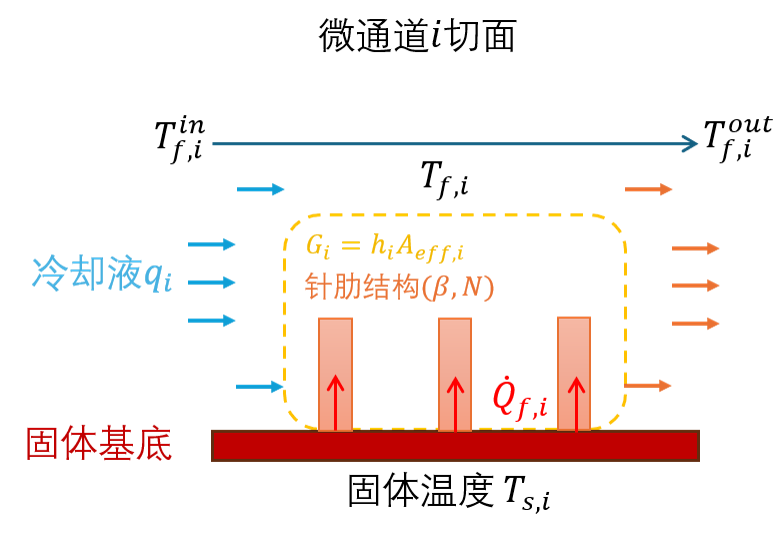
\includegraphics[width=0.72\textwidth]{fig_q1_local_heat_transfer.png}
\caption{第 $i$ 条微通道对应区域内的换热关系。冷却液以流量 $q_i$ 进入针肋区，其代表温度由 $T_{f,i}^{\mathrm{in}}$ 升至 $T_{f,i}^{\mathrm{out}}$。针肋结构 $(\beta,N)$ 和支路流量共同决定 $G_i=h_iA_{\mathrm{eff},i}$。固体向冷却液传热，传热率记为 $\dot Q_{f,i}$。图中针肋数量仅作示意。}
\label{fig:q1-local-heat-transfer}
\end{figure}

将换热系数与有效换热面积合并记为
\begin{equation}
G_i=h_iA_{\mathrm{eff},i},\qquad
\dot Q_{f,i}=G_i(T_{s,i}-T_{f,i}).
\end{equation}
$G_i$ 的单位为 $\mathrm{W\,K^{-1}}$，表示传热率与固液温差之比。$G_i$ 越大，同样温差下能够传递的热量越多。即使结构参数相同，支路流量不同也会因流速和边界层的差异而改变换热。以平均支路流量 $\bar q$ 为基准，将此时的 $G_i$ 记为 $G_0(\beta,N)$。支路流量偏离 $\bar q$ 所产生的影响用无量纲函数 $\psi(q_i/\bar q)$ 表示，并令 $\psi(1)=1$。于是
\begin{equation}
G_i=G_0(\beta,N)\psi\!\left(\frac{q_i}{\bar q}\right).
\end{equation}
冷却液进出该区域的能量守恒关系为
\begin{equation}
\dot m_i c_p(T_{f,i}^{\mathrm{out}}-T_{f,i}^{\mathrm{in}})
=\dot Q_{f,i},\qquad \dot m_i=\rho q_i
\end{equation}
其中，$T_{f,i}^{\mathrm{in}}$ 是冷却液由入口歧管进入第 $i$ 个微通道时的温度，$T_{f,i}^{\mathrm{out}}$ 是其穿过针肋区并进入出口歧管时的温度。在本题所处的流量范围内，支路流量偏低会削弱局部换热。在热负荷相近时，冷却液温升也会增大，相应区域更容易出现高温。

\subsubsection{芯片与衬底的温度分布}
只按支路分别计算温度会忽略不同区域之间的固体导热。芯片热源位于中央 $6\,\mathrm{mm}\times6\,\mathrm{mm}$ 区域。某处冷却较弱时，热量仍会沿芯片和衬底向周围传导，因此温度非均匀性不能只由各支路的流体温升决定。Lee 等（2024）的一维模型同时考虑了固体沿流向导热以及固体与冷却液之间的换热\cite{Lee2024}。借鉴这一做法，本文假定各层接触良好，把芯片和衬底近似为二维导热区域，并用厚度方向的平均温度表示各位置的固体温度，从而保留两个平面方向上的热扩散。图~\ref{fig:q1-temperature-field} 标出了热源区域、各微通道对应区域、平面内导热和边界条件。

\begin{figure}[H]
\centering
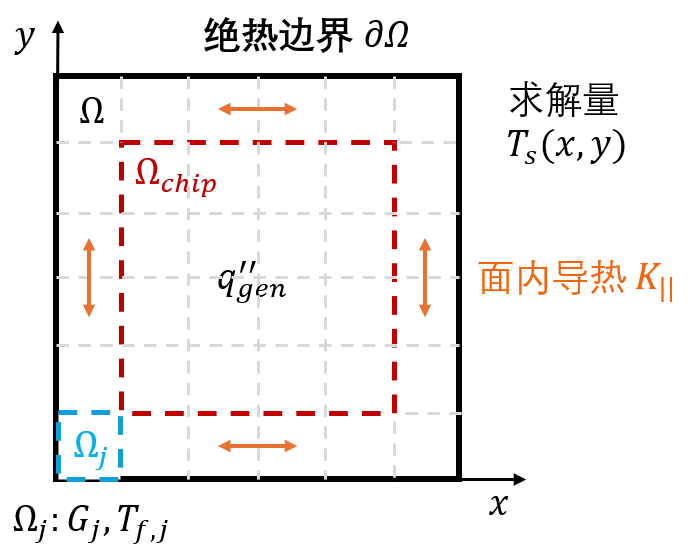
\includegraphics[width=0.62\textwidth]{fig_q1_temperature_field.png}
\caption{芯片与衬底的二维导热示意。$\Omega$ 为整个散热区域，中央 $\Omega_{\mathrm{chip}}$ 为芯片热源投影区域，面热源为 $q''_{\mathrm{gen}}$；每个区域 $\Omega_j$ 的 $G_j$ 表示传热率与固液温差之比，$T_{f,j}$ 为冷却液代表温度。$K_{\parallel}$ 表示固体的面内导热参数，外边界 $\partial\Omega$ 采用绝热条件，待求的是固体温度场 $T_s(x,y)$。}
\label{fig:q1-temperature-field}
\end{figure}

各层沿平面方向的导热参数按厚度累加为
\begin{equation}
K_{\parallel}=\sum_{\ell}k_{\parallel,\ell}^{\mathrm{eff}}t_{\ell},
\end{equation}
其中 $k_{\parallel,\ell}^{\mathrm{eff}}$ 和 $t_\ell$ 分别为第 $\ell$ 层沿平面方向的等效导热系数与厚度，连续实体层取相应材料的导热系数。对于含微通道和针肋的区域，$k_{\parallel,\ell}^{\mathrm{eff}}$ 表示固体结构经平面平均后的导热系数，冷却液带走的热量另由 $g(x,y)$ 描述。$K_{\parallel}$ 的量纲为 $\mathrm{W\,K^{-1}}$。上述关系首先用于所取的一组歧管及其相连微通道。若局部压力和几何参数已知，其余重复区域可采用同样的方法计算，并映射到整个散热面。厚度平均后的稳态能量守恒方程为
\begin{equation}
-\nabla_{\parallel}\!\cdot\!\left(K_{\parallel}\nabla_{\parallel}T_s\right)
+g(x,y)[T_s(x,y)-T_f(x,y)]=q''_{\mathrm{gen}}(x,y).
\label{eq:pde}
\end{equation}
式~\eqref{eq:pde} 中，第一项表示热量在芯片和衬底平面内的传导，第二项表示冷却液带走的热量，右端表示芯片产生的热量。在每个微通道对应区域内，$T_f(x,y)$ 取该区域冷却液的代表温度 $T_{f,j}$。
外边界采用绝热条件
\begin{equation}
\vect n\cdot K_{\parallel}\nabla_{\parallel}T_s=0,\qquad (x,y)\in\partial\Omega,
\end{equation}
这与主模型中忽略外表面散热的假设一致。将整个散热区域划分为若干小区域，记第 $j$ 个区域为 $\Omega_j$。该区域的 $G_j$ 满足
\begin{equation}
G_j=\int_{\Omega_j}g(x,y)\,\mathrm dA.
\end{equation}
其中，$g(x,y)$ 表示各位置单位面积上的传热率与固液温差之比，单位为 $\mathrm{W\,m^{-2}K^{-1}}$。歧管本身不直接出现在二维方程中，其影响通过微通道流量和相应区域的 $G_j$ 传递给 $g(x,y)$。温度场确定后，即可计算整体热阻和温度非均匀性。
局部流量偏低通常会削弱换热并增大冷却液温升，使对应区域更易升温。不过，芯片和衬底中的横向导热会在区域之间重新分配热量，因此支路流量差异与温度分布不均匀程度之间并无固定比例关系。Pu 等（2024）对歧管式微通道温度分布的数值研究也观察到类似现象\cite{Pu2024}。

\subsection{数据检验与影响规律}
\subsubsection{压降关系检验}
下面利用总体性能数据检验前述尺度关系。4 个无针肋样本满足
\begin{equation}
\Pstar_0=0.04312+0.72692\eta^{-2},\qquad
R^2=0.99995,\quad \mathrm{RMSE}=1.24\times10^{-4}.
\end{equation}
在附件给出的 $\eta$ 范围内，该关系对 4 个无针肋样本的拟合误差很小。由于样本数有限，本文不将其推广为系统总压降的一般公式。

为比较几种针肋尺寸与排数的组合方式，对每个组合量 $X$ 均拟合 $\Pstar=a_0+a_1\eta^{-2}+a_2X$，无针肋样本取 $X=0$。附件 2 全部 84 组样本的拟合结果见表~\ref{tab:congestion}。
\begin{table}[H]
\centering
\caption{不同针肋组合量的压降拟合结果}
\label{tab:congestion}
\begin{tabular}{lcc}
\toprule
组合量 & $R^2$ & RMSE\\
\midrule
$N\beta$ & 0.9170 & 0.00795\\
$N\beta^2$ & 0.9764 & 0.00424\\
$N\beta/(1-\beta)$ & 0.9535 & 0.00595\\
$N\beta^2/(1-\beta)$ & 0.9777 & 0.00412\\
\bottomrule
\end{tabular}
\end{table}
$N\beta^2/(1-\beta)$ 的误差略小，但其 $R^2$ 与 $N\beta^2$ 仅相差约 0.0013。两者精度接近，而 $N\beta^2$ 的几何含义更直接，故后文采用这一组合量。令无针肋点满足 $N\beta^2=0$，并与有针肋样本共同拟合，得到
\begin{equation}
\Pstar_{\mathrm{fit}}=0.03841+0.74439\eta^{-2}+0.09077N\beta^2,
\end{equation}
其 $R^2=0.9764$、RMSE 为 0.00424。这里的 $R^2$ 对应同时包含 $\eta^{-2}$ 和 $N\beta^2$ 的拟合式，并非 $N\beta^2$ 的单变量拟合结果。该简化关系只用于概括压降的主要变化趋势。后续数值预测仍采用问题二建立的模型。

\subsubsection{三个参数的影响}
80 个有针肋样本覆盖全部 $4\times4\times5$ 个参数组合。分别固定一个参数，并对其余组合取平均，结果见表~\ref{tab:means}。

\begin{table}[H]
\centering
\caption{各参数水平下三项指标的平均值}
\label{tab:means}
\begin{tabular}{ccccc}
\toprule
参数 & 水平 & 平均 $\Rstar$ & 平均 $\Pstar$ & 平均 $\Ustar$\\
\midrule
\multirow{4}{*}{$\beta$} & 0.10 & 0.753881 & 0.104692 & 0.820108\\
 & 0.15 & 0.745996 & 0.107705 & 0.811081\\
 & 0.20 & \textbf{0.738920} & 0.112094 & \textbf{0.799620}\\
 & 0.30 & 0.745610 & 0.143717 & 0.821918\\
\midrule
\multirow{4}{*}{$\eta$} & 3.0 & \textbf{0.737264} & 0.143255 & 0.825196\\
 & 3.5 & 0.743543 & 0.120811 & \textbf{0.805476}\\
 & 4.0 & 0.752004 & 0.106945 & 0.810177\\
 & 4.5 & 0.751597 & \textbf{0.097196} & 0.811877\\
\midrule
\multirow{5}{*}{$N$} & 2 & 0.757179 & \textbf{0.100285} & 0.807209\\
 & 4 & 0.746221 & 0.107326 & \textbf{0.795144}\\
 & 6 & 0.743284 & 0.118482 & 0.809099\\
 & 8 & 0.743165 & 0.127893 & 0.827115\\
 & 10 & \textbf{0.740660} & 0.131274 & 0.827341\\
\bottomrule
\end{tabular}
\parbox{0.82\textwidth}{\footnotesize 注：粗体表示同一参数下对应指标的最优均值。}
\end{table}

针肋宽度比从 0.10 增至 0.20 时，平均热阻和温度非均匀性均有所下降。增至 0.30 后，两者重新升高，平均压降也由 0.112094 增至 0.143717。适度增粗针肋有利于换热，直径继续增大则会明显压缩通流空间，并增加绕流损失。

歧管深高比对压降的影响最为明显。$\eta$ 从 3.0 增至 4.5 时，平均压降由 0.143255 降至 0.097196，降幅为 32.2\%，与前述 $\eta^{-2}$ 关系的变化方向一致。热阻却没有随 $\eta$ 单调下降，温度非均匀性也在 $\eta=3.5$ 附近取得较低均值。这是因为歧管高度不仅影响总体压降，还会改变各微通道的流量分配和局部换热。

针肋排数由 2 增至 10 后，平均热阻从 0.757179 降至 0.740660，平均压降则由 0.100285 升至 0.131274。温度非均匀性在 $N=4$ 时达到最低均值 0.795144，随后重新升高。增加针肋排数总体上能够降低热阻，却不会持续改善温度均匀性。

附件给出的结果是确定性的数值数据，每个参数组合也只有一次结果，因此本文不作基于随机误差的显著性检验，只比较各参数主效应平方和占总平方和的比例。对任一指标 $y$ 和参数 $x\in\{\beta,\eta,N\}$，记 $x$ 有 $L_x$ 个水平，每个水平对应 $m_x$ 个其他参数组合，$\bar y_{x_r}$ 为第 $r$ 个水平的指标均值，$\bar y$ 为全部 80 个样本的均值，则
\begin{equation}
SS_x=m_x\sum_{r=1}^{L_x}\left(\bar y_{x_r}-\bar y\right)^2,
\qquad
SS_T=\sum_{i=1}^{80}(y_i-\bar y)^2.
\label{eq:main-effect-ss}
\end{equation}
本题中 $m_\beta=m_\eta=20$，$m_N=16$。图~\ref{fig:q1-mechanism-validation}(b) 绘制的是 $100SS_x/SS_T\%$，其余部分由参数之间的交互作用构成。$\eta$ 对压降的主效应平方和占总平方和的 38.89\%，$N$ 对温度非均匀性的对应比例为 48.00\%。压降中的 $\beta\times N$ 交互项另占 11.25\%。为单独观察针肋部分的变化，从 $P^*$ 中减去拟合得到的 $\eta^{-2}$ 项：
\begin{equation}
P_{\mathrm{corr}}^*=P^*-0.74439\eta^{-2}.
\end{equation}

\begin{figure}[H]
\centering
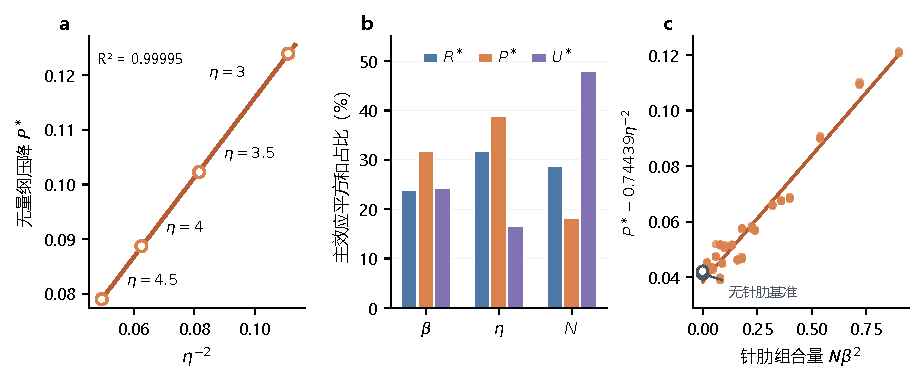
\includegraphics[width=\textwidth]{fig_q1_mechanism_validation.pdf}
\caption{问题一的压降关系与数据检验。（a）无针肋压降与 $\eta^{-2}$ 的关系；（b）三个参数主效应的平方和占比；（c）减去 $\eta^{-2}$ 项后的 $P^*$ 与 $N\beta^2$ 的关系。灰色空心点表示无针肋基准。}
\label{fig:q1-mechanism-validation}
\end{figure}

表~\ref{tab:q1-influence} 汇总了三个结构参数对各项性能的主要影响及其物理解释。其中“先降后升”和“非单调”仅指附件覆盖范围内的变化，不外推至更宽的几何区间。
\begin{table}[H]
\centering
\caption{三个结构参数对三项性能指标的主要影响规律}
\label{tab:q1-influence}
\small
\begin{tabularx}{\textwidth}{c c c c X}
\toprule
参数变化 & $\Rstar$ & $\Pstar$ & $\Ustar$ & 主要原因\\
\midrule
$\beta\uparrow$ & 先降后升 & 上升 & 先降后升 & 换热面积和边界层扰动增强，但针肋变粗后，可供水流通过的空间减小，绕流损失也增大\\
$\eta\uparrow$ & 非单调 & 明显下降 & 非单调 & 歧管截面增大、平均流速降低，同时各微通道获得的流量也发生变化\\
$N\uparrow$ & 总体下降 & 上升 & 先改善后恶化 & 换热面积增加，但针肋越多，总阻力越大，后排针肋还会受到前排尾流影响\\
\bottomrule
\end{tabularx}
\end{table}

\subsubsection{为什么要同时考虑三个指标}
$\Rstar$ 反映整体散热水平。流量固定时，压降越大，所需泵功通常越高。$\Ustar$ 则反映温度分布的均匀程度。附件样本中，三项指标的最小值分别出现在不同结构上：
\begin{table}[H]
\centering
\caption{附件样本中的三个单目标最小值}
\begin{tabular}{lcc}
\toprule
目标 & 样本最小值 & 对应 $(\beta,\eta,N)$\\
\midrule
$\Rstar$ & 0.721922 & $(0.20,3.0,10)$\\
$\Pstar$ & 0.076688 & $(0.20,4.5,2)$\\
$\Ustar$ & 0.774010 & $(0.20,4.5,4)$\\
\bottomrule
\end{tabular}
\end{table}
三个最优结构互不相同，说明降低热阻并不能同时保证较小的压降和较均匀的温度分布。例如，增加针肋通常会强化换热，却也会增大流动阻力，后续优化必须在三项指标之间作出取舍。前述模型把结构参数与流量分配、局部换热和固体导热联系起来，说明了三项性能变化的物理原因。由于局部关系缺少定参数据，下一节再用响应面计算结构参数与三项指标之间的定量关系。

\section{问题二：性能预测模型}
\subsection{数据处理}
4 个无针肋样本均位于 $(\beta,N)=(0,0)$，附件没有 $\beta>0,N=0$ 或 $\beta=0,N>0$ 等过渡组合。若将它们与其余 80 个样本共同拟合，模型需要在没有数据支持的区域描述从无针肋到有针肋的变化。因此，无针肋点只用于问题一的基准比较，问题二使用其余 80 个有针肋样本，其参数水平为
\begin{equation*}
\beta\in\{0.10,0.15,0.20,0.30\},\quad
\eta\in\{3.0,3.5,4.0,4.5\},\quad N\in\{2,4,6,8,10\}.
\end{equation*}
程序检查了 84 组数据的缺失与重复情况，并确认 80 个有针肋样本覆盖全部参数组合。数据处理中不删除异常点，也不对指标值作平滑处理。由于三个设计变量的数值尺度不同，高次多项式直接使用原始变量会使设计矩阵各列相差较大，故先作平移和缩放：
\begin{equation}
x_1=\frac{\beta-0.20}{0.10},\qquad
x_2=\frac{\eta-3.75}{0.75},\qquad
x_3=\frac{N-6}{4}.
\label{eq:encoding}
\end{equation}

\subsection{模型比较}
本题只有三个设计变量，样本又位于规则参数网格上，适合用参数较少的多项式响应面描述平滑的非线性变化\cite{BoxWilson1951,He2024}。候选模型取二次和三次多项式响应面，后文简称二次响应面和三次响应面。由于 $\beta$ 和 $\eta$ 各只有 4 个水平，四次项无法与三次及以下项独立区分，当前数据不能唯一确定完整四次响应面的系数，故不再比较更高阶模型。

另选取 Mat\'ern-$5/2$ 核和径向基函数（RBF）核的高斯过程作为非参数对照\cite{RasmussenWilliams2005}，以判断三次响应面的误差优势是否依赖多项式形式。两种模型采用相同的五折划分计算预测误差。Lee 等（2026）曾把简化模型与三维计算流体力学（CFD）结果结合，用不同精度的数据共同训练预测模型\cite{Lee2026}。本题没有可配对的第二套数据，因而不采用这种方法。

\subsection{五折交叉验证与模型选择}
若随机划分样本，一个验证点附近往往仍有许多参数十分接近的训练样本，使验证误差偏小。但删除一个 $\beta$ 或 $\eta$ 水平后只剩 3 个不同水平，又无法单独确定该变量的所有三次项。为兼顾这两点，令 $i_\beta,i_\eta,i_N$ 分别为三个参数水平从 0 开始的编号，按
\begin{equation*}
s=(i_\beta+2i_\eta+3i_N)\bmod5
\end{equation*}
分成 5 折。每折包含 16 个分散的参数组合，并覆盖各因素的全部水平。两种高斯过程均采用式~\eqref{eq:encoding} 的编码输入，各指标在每个训练折内分别标准化。核函数写为常数幅值与 Mat\'ern-$5/2$ 或 RBF 核的乘积，再叠加白噪声项。核幅值、三个方向的长度尺度和白噪声强度通过最大化对数边际似然估计，优化时额外使用 2 组随机初值。随机种子和超参数边界见随附代码。
\begin{table}[H]
\centering
\caption{不同预测模型的五折交叉验证 RMSE}
\label{tab:cv}
\begin{tabular}{lccc}
\toprule
模型 & $\Rstar$ & $\Pstar$ & $\Ustar$\\
\midrule
二次响应面 & $4.382\times10^{-3}$ & $3.008\times10^{-3}$ & $8.468\times10^{-3}$\\
三次响应面 & $3.459\times10^{-7}$ & $5.588\times10^{-4}$ & $3.005\times10^{-4}$\\
Mat\'ern-$5/2$ 高斯过程 & $2.666\times10^{-4}$ & $8.023\times10^{-4}$ & $7.908\times10^{-4}$\\
RBF 高斯过程 & $3.961\times10^{-6}$ & $1.135\times10^{-3}$ & $1.167\times10^{-3}$\\
\bottomrule
\end{tabular}
\end{table}
表~\ref{tab:cv} 显示，三次响应面的交叉验证误差均低于二次响应面，两种高斯过程也未在任一指标上取得更小的 RMSE。其 $\Rstar$ 交叉验证 RMSE 为 $3.46\times10^{-7}$，已接近附件保留至小数点后六位的记录精度，说明当前规则网格上的 $\Rstar$ 随参数变化较为平滑，三次响应面足以描述这些样本。后续计算采用三次响应面。

\subsection{最终模型与预测检验}
对任一指标 $y\in\{\Rstar,\Pstar,\Ustar\}$，最终模型写为
\begin{equation}
\hat y(\vect x)=\sum_{a+b+c\leq3}\theta_{abc}x_1^a x_2^b x_3^c.
\label{eq:cubic}
\end{equation}
式~\eqref{eq:cubic} 中 $a,b,c\in\mathbb Z_{\geq0}$，共含 20 项。三项指标的响应面分别用最小二乘法估计，编码后设计矩阵的条件数为 14.17，全部拟合系数列于附录表~\ref{tab:cubic-coefficients}。表~\ref{tab:fit} 中的训练集指标用于核对模型对现有数据的拟合程度，不能代替交叉验证结果。表中还列出了平均绝对误差（MAE）。
\begin{table}[H]
\centering
\caption{三次响应面的训练集拟合指标}
\label{tab:fit}
\begin{tabular}{lccc}
\toprule
指标 & $R^2$ & RMSE & MAE\\
\midrule
$\Rstar$ & $\approx1.0000$ & $2.416\times10^{-7}$ & $2.045\times10^{-7}$\\
$\Pstar$ & 0.9997822 & $4.094\times10^{-4}$ & $1.636\times10^{-4}$\\
$\Ustar$ & 0.9998247 & $2.375\times10^{-4}$ & $1.119\times10^{-4}$\\
\bottomrule
\end{tabular}
\end{table}

表~\ref{tab:q2-validation-summary} 汇总了四种验证结果。第三种检验依次留出 $N=4,6,8$ 的全部样本，再合并各次预测误差，以检查模型对训练中未出现过的中间排数能否保持预测精度。第四种检验整体留出 $\beta\in\{0.15,0.20\}$、$\eta\in\{3.5,4.0\}$ 且覆盖全部五个已观测 $N$ 水平的 20 组样本，因此这一局部区域内相邻的 $(\beta,\eta)$ 组合均不参与拟合。
\begin{table}[H]
\centering
\caption{三次响应面的四类预测检验 RMSE}
\label{tab:q2-validation-summary}
\begin{tabular}{lccc}
\toprule
检验方式 & $\Rstar$ & $\Pstar$ & $\Ustar$\\
\midrule
五折交叉验证 & $3.459\times10^{-7}$ & $5.588\times10^{-4}$ & $3.005\times10^{-4}$\\
留一交叉验证 & $3.296\times10^{-7}$ & $5.476\times10^{-4}$ & $2.976\times10^{-4}$\\
留出整个 $N$ 水平 & $3.181\times10^{-7}$ & $7.383\times10^{-4}$ & $3.591\times10^{-4}$\\
留出中央 20 组相邻参数 & $4.047\times10^{-7}$ & $2.983\times10^{-4}$ & $4.284\times10^{-4}$\\
\bottomrule
\end{tabular}
\end{table}
四种验证所得误差均与训练误差处于相近量级。即使把中央 20 组相邻参数组合全部留出，三项 RMSE 仍不超过 $4.29\times10^{-4}$，说明较低误差并不只是因为验证点附近保留了相邻训练样本。因此，在附件覆盖的参数范围内，三次响应面没有表现出明显的过拟合。这些结果只说明模型在参数范围内的插值能力，不能用来判断范围外预测或真实实验误差。
图~\ref{fig:q2-surrogate-validation}(b)--(d) 展示五折交叉验证中未参与拟合样本的预测结果。

\begin{figure}[H]
\centering
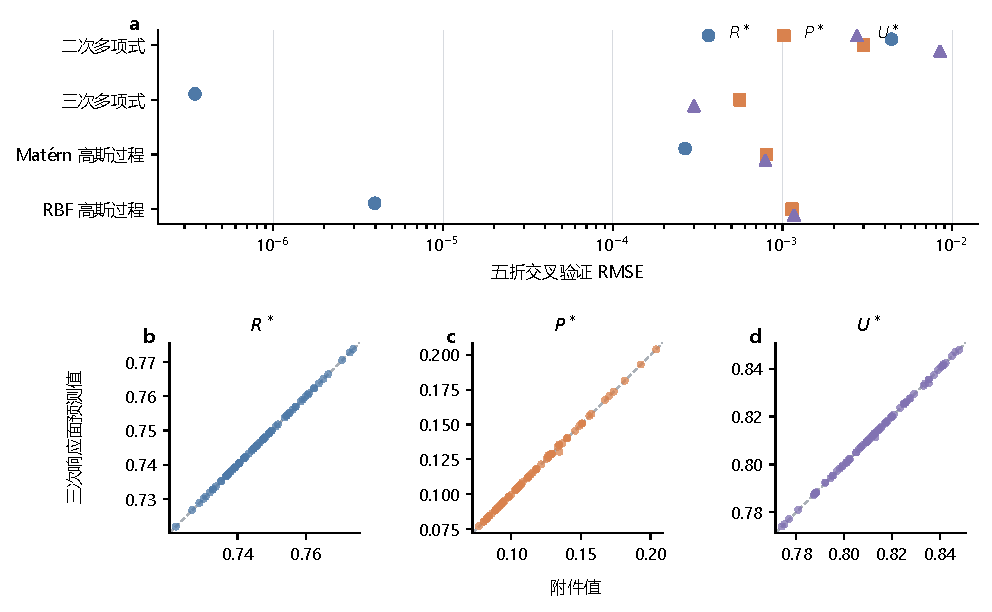
\includegraphics[width=\textwidth]{fig_q2_surrogate_validation.pdf}
\caption{预测模型的选择与验证。（a）四种模型的五折交叉验证 RMSE；（b）--（d）三次响应面在各验证折上的预测值与附件值。灰色虚线表示理想预测关系。}
\label{fig:q2-surrogate-validation}
\end{figure}

较低的预测误差并不能保证模型给出合理的变化方向。因此，在密集网格上令 $\beta$、$\eta$ 各取 81 个等距点，并遍历 $N=2,3,\ldots,10$，得到
\begin{equation*}
\frac{\partial\hat P^*}{\partial\eta}\in[-0.0575,-0.0171],
\end{equation*}
即预测压降始终随 $\eta$ 增大而下降。后续优化采用由全部 80 组样本重新估计的三次响应面。

\begin{figure}[H]
\centering
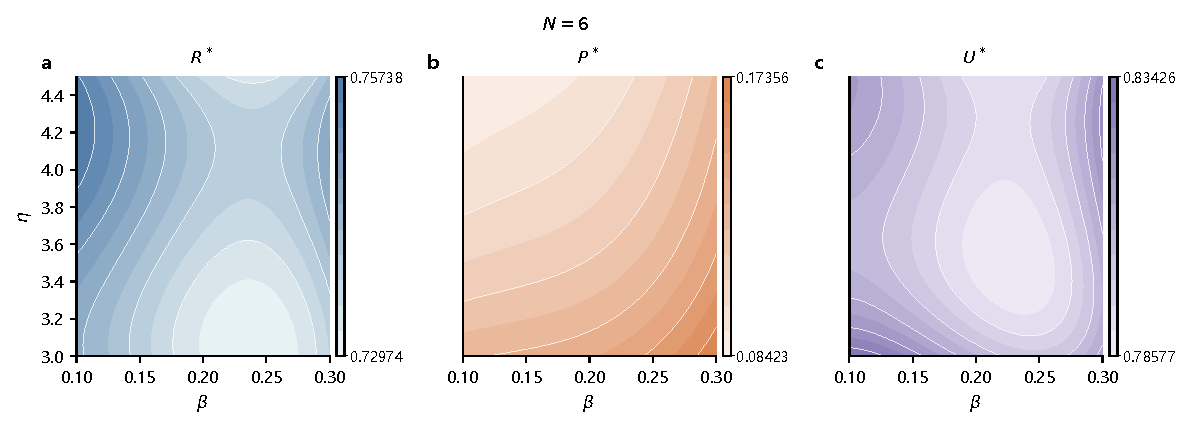
\includegraphics[width=\textwidth]{fig_q2_response_surfaces.pdf}
\caption{$N=6$ 时三项指标随 $\beta$、$\eta$ 的预测结果。（a）--（c）分别为 $\Rstar$、$\Pstar$ 和 $\Ustar$。}
\label{fig:q2-response-surfaces}
\end{figure}

图~\ref{fig:q2-response-surfaces} 给出了 $N=6$ 时三次响应面随 $\beta$、$\eta$ 的变化。压降 $\Pstar$ 随 $\eta$ 增大总体下降，与问题一的分析一致。$\Rstar$ 和 $\Ustar$ 对 $\beta$、$\eta$ 呈非单调变化。三项指标的低值区域并不重合，同一组结构参数无法使三项性能同时达到各自最优，因而需要在下一节比较不同目标之间的取舍。

\section{问题三：多目标优化}
\subsection{参数范围与单项最优结果}
已有微通道结构优化研究常用响应面或 Kriging 模型预测性能，再通过多目标搜索筛选 Pareto 前沿\cite{He2024,Rong2026}。本题只有两个连续变量，$N$ 也只取有限个整数，因此可逐一枚举 $N$，在 $(\beta,\eta)$ 网格上直接筛选 Pareto 方案。单项最优值和综合方案使用差分进化算法搜索\cite{StornPrice1997}，随机种子固定，以便复核计算结果。

允许搜索的参数范围记为 $\mathcal X$：
\begin{equation}
\mathcal X=\{(\beta,\eta,N):0.10\leq\beta\leq0.30,
\ 3.0\leq\eta\leq4.5,
\ N\in\{2,3,\ldots,10\}\}.
\end{equation}
附件只给出了偶数排数，但从结构上看，$N$ 可以取任意整数。问题二在留出整个 $N$ 水平时仍得到较低预测误差，后续搜索范围因此取 $N=2,3,\ldots,10$。其中 $N=3,5,7,9$ 没有直接观测数据，相应结果是响应面对奇数排数的插值，而不是附件已有的结构组合。为判断推荐方案是否依赖这一插值，后文还将只保留偶数排数重新计算。
对每个整数 $N$，在 $(\beta,\eta)$ 平面按 $\Delta\beta=0.001$、$\Delta\eta=0.01$ 的规则网格计算三项指标。如果另一方案在三项指标上均不差于当前方案，且至少一项更优，则删除当前方案。将各 $N$ 下保留的设计合并后再次筛选，得到 Pareto 候选集。计算三个单项最优值和后文的综合方案时，对每个整数 $N$ 使用差分进化搜索连续参数，再在所得结果附近进行有界局部优化。三个单项最优值见表~\ref{tab:ideal-designs}。
\begin{table}[H]
\centering
\caption{响应面给出的三个单目标最优设计}
\label{tab:ideal-designs}
\begin{tabular}{lcc}
\toprule
目标 & 最小值 & 对应 $(\beta,\eta,N)$\\
\midrule
$\Rstar$ & 0.720227 & $(0.2320,3.0677,10)$\\
$\Pstar$ & 0.076048 & $(0.2286,4.5000,2)$\\
$\Ustar$ & 0.770827 & $(0.2242,4.5000,3)$\\
\bottomrule
\end{tabular}
\end{table}
三个单项最优值组成理想点 $\vect f^I=(0.720227,0.076048,0.770827)$，离散 Pareto 前沿上各分量的最大值作为归一化参考上界 $\vect f^{\mathrm{ref}}=(0.760203,0.158829,0.819280)$。三项指标虽然都是无量纲数，在当前参数范围内的变化幅度仍不相同，直接比较原始数值会受到尺度影响。按理想值到参考上界的区间归一化：
\begin{equation}
z_j=\frac{f_j-f_j^I}{f_j^{\mathrm{ref}}-f_j^I},\qquad j\in\{R,P,U\}.
\label{eq:q3-normalization}
\end{equation}

\subsection{综合方案}
题目没有说明三项指标的优先级。即使三个权重均取 $1/3$，加权和仍可能允许某一项明显恶化，再由另外两项予以补偿。为控制偏离理想点最远的指标，本文采用 Chebyshev 标量化方法\cite{Miettinen1998}，在上述参数范围内最小化三项归一化偏差的最大值：
\begin{equation}
\min_{(\beta,\eta,N)\in\mathcal X}D_\infty
=\min_{(\beta,\eta,N)\in\mathcal X}\max\{z_R,z_P,z_U\}.
\end{equation}
计算得到的连续优化值为
\begin{equation}
(\beta,\eta,N)=(0.22494,4.50000,6),
\end{equation}
三项指标及归一化偏差分别为
\begin{equation}
(\Rstar,\Pstar,\Ustar)=(0.734329,0.097999,0.790190),
\qquad \vect z=(0.3528,0.2652,0.3996).
\end{equation}
原始样本中的 $\beta$ 水平间距较大，因此工程推荐写为 $\beta\approx0.225$、$\eta=4.50$、$N=6$。数值 0.22494 仅用于复核优化结果。还需注意，$\eta=4.50$ 位于当前数据范围的上边界。
为检查归一化参考上界是否依赖网格步长，将 Pareto 网格加密至 $\Delta\beta=0.0005$、$\Delta\eta=0.005$。重新计算得到
\[
\vect f^{\mathrm{ref}}=(0.760176,0.158616,0.819280).
\]
Chebyshev 方案仍为 $(0.22494,4.50,6)$，三项指标没有变化，$D_\infty$ 仍为 0.39963。两档网格得到的推荐结果一致，参考上界的微小变化没有影响最终方案。
只允许附件出现过的偶数排数时结果不变。作为对照，再以理想点的欧氏距离
\begin{equation}
D_2=\sqrt{z_R^2+z_P^2+z_U^2}
\end{equation}
评价综合性能。此时最优排数变为 $N=5$，$\beta=0.22430$、$\eta=4.50$，对应指标值为 $(0.736547,0.091368,0.779149)$。最大偏差最小准则和欧氏距离准则分别选择 $N=6$、$N=5$。两种结果都集中在 5--6 排，表明排数的选择会受到折中准则影响。$\eta=4.5$ 已是数据范围的上界，因而这里只能认为，在附件给出的 $\eta\in[3,4.5]$ 内，较大的歧管深高比更有利于当前综合目标。$\eta>4.5$ 后的趋势无法由现有数据判断。

\begin{figure}[H]
\centering
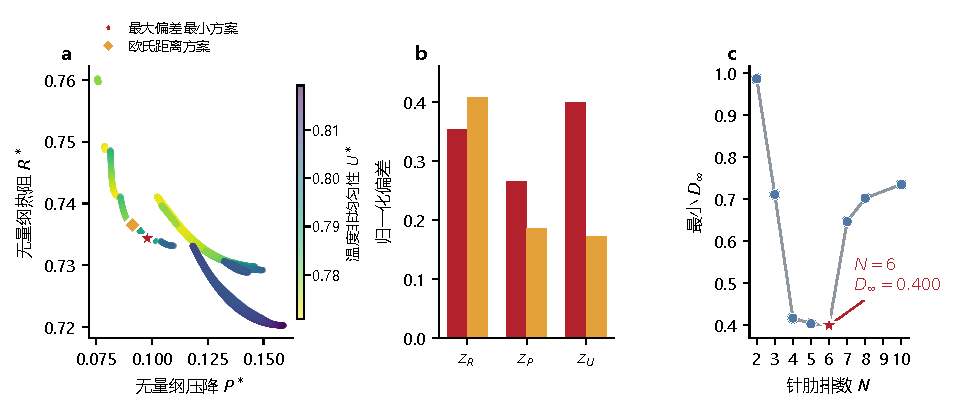
\includegraphics[width=\textwidth]{fig_q3_pareto_compromise.pdf}
\caption{多目标优化结果。（a）Pareto 前沿的二维投影；（b）最大偏差最小方案与欧氏距离方案的归一化偏差；（c）各整数排数下的最小最大偏差 $D_\infty$。红色星号表示最大偏差最小方案，橙色菱形表示欧氏距离方案。}
\label{fig:q3-pareto-compromise}
\end{figure}

图~\ref{fig:q3-pareto-compromise}(b) 中，最大偏差最小方案牺牲了部分压降性能，三项偏差因而更为均衡。图~\ref{fig:q3-pareto-compromise}(c) 中 $N=6$ 的最小 $D_\infty$ 最低，推荐排数并非由某一项指标单独决定。

\section{问题四：权重变化下的方案选择}
\subsection{使方案最优的权重范围}
问题三没有预设指标权重，以三项归一化偏差中的最大值选择方案。问题四改为考察权重变化，判断应用侧重点不同时，哪些设计仍可能成为最优方案。

候选方案取问题三按 $\Delta\beta=0.001$、$\Delta\eta=0.01$ 得到的 4293 个 Pareto 网格点，已被支配的设计不再参与权重比较。令 $\vect w=(w_R,w_P,w_U)$，权重满足
\begin{equation}
\Delta_2=\{\vect w:w_R,w_P,w_U\geq0,\ w_R+w_P+w_U=1\}.
\end{equation}
三项非负权重之和为 1，所有组合可表示在一个三角形内。为避免指标变化幅度不同而扭曲权重的实际作用，问题四继续使用式~\eqref{eq:q3-normalization} 中的 $z_R$、$z_P$、$z_U$ 进行加权。给定权重后，设计 $i$ 的得分为 $V_i(\vect w)=\vect w^{\mathsf T}\vect z_i$，得分越小，综合性能越好。使设计 $i$ 成为最优的权重范围为
\begin{equation}
\mathcal W_i=\{\vect w\in\Delta_2:\vect w^{\mathsf T}(\vect z_i-\vect z_k)\leq0,\ \forall k\}.
\end{equation}
这些线性不等式在权重三角形内确定了设计 $i$ 的最优区域 $\mathcal W_i$。该区域占整个三角形的面积比例记为
\begin{equation}
B_i=\frac{\operatorname{Area}(\mathcal W_i)}{\operatorname{Area}(\Delta_2)}.
\end{equation}
Tervonen 和 Lahdelma（2007）提出的随机多准则可接受性分析（SMAA）也考察了不同权重下方案的可接受程度\cite{Tervonen2007}。本题各候选方案的指标已经确定，采用线性加权时可以直接求出相应区域。题目没有提供权重依据，计算中也不额外偏向某类权重组合。$B_i$ 越大，表示该设计能在更多权重组合下成为最优，但面积占比不能解释为实际发生概率。参数网格取 $\Delta\beta=0.001$、$\Delta\eta=0.01$，$N$ 为 2--10 的整数。这些步长只用于计算，不代表制造公差。

\subsection{结果与稳定性检查}
575 个候选方案可在部分权重组合下成为最优。其中，$(0.224,4.50,4)$ 的单点权重范围最大，占整个权重三角形的 5.23\%，对应的 $\Rstar$、$\Pstar$ 和 $\Ustar$ 分别为 0.741114、0.085117 和 0.771783。网格加密后，同一片参数范围会被更多候选点分割，这一单点比例也会随网格步长改变。由于排名靠前的方案集中在 $\beta\approx0.22$、$\eta=4.5$、$N=3$--$4$，下面将邻近设计合并后再作统计。

权重三角形三个顶点对应的设计与单目标结果一致。$w_R=1$ 时选择 $N=10$ 的低热阻方案，$w_P=1$ 时选择 $N=2$、$\eta=4.5$ 的低压降方案，$w_U=1$ 时选择 $N=3$、$\eta=4.5$ 的温度最均匀方案。当评价重点从热阻转向压降或温度均匀性，最优排数也从较大的 $N$ 转向 $N=2$--$4$。为减小单个网格点对步长的依赖，再按相同 $N$ 合并统计：
\begin{equation}
B_N=\sum_{i:N_i=N}B_i.
\end{equation}
其中 $N=4$、3、10 和 5 的总权重占比依次为 47.17\%、28.76\%、12.36\% 和 9.10\%。区域边界只由主网格确定。先取 $B_N$ 合计最大的相邻排数组合，得到 $N=3$--$4$，再取这两种排数下总权重面积最大的 $\eta=4.5$。最后从主网格的 $\beta$ 节点中选择最窄连续区间，使其包含主网格中单点权重范围最大的设计，且累计覆盖至少 50\% 的权重组合。最终得到
\begin{equation}
\mathcal C=\{(\beta,\eta,N):0.215\leq\beta\leq0.224,\ \eta=4.5,\ N\in\{3,4\}\},
\end{equation}
并令 $B_{\mathcal C}=\sum_{i\in\mathcal C}B_i$。主网格中 $B_{\mathcal C}=51.66\%$。因此，推荐结果应理解为一组相近参数，而不是某个精确网格点。

区域 $\mathcal C$ 确定后保持边界不变，再进行两组独立复算。只保留附件直接观测的 $N\in\{2,4,6,8,10\}$ 时，$N=3$ 不再参与比较，区域内 $N=4$ 设计的权重占比为 48.38\%。将连续网格加密至 $\Delta\beta=0.0005$、$\Delta\eta=0.005$ 后，单点最大比例由 5.23\% 降至 2.77\%，固定区域的占比为 49.99\%。两项复算均接近主网格的 51.66\%，说明网格设置会改变单点面积，但优势设计仍集中在同一参数邻域。
\begin{table}[H]
\centering
\caption{主网格所定区域 $\mathcal C$ 在两种离散设置下的独立复算}
\label{tab:q4-stability}
\small
\begin{tabularx}{\textwidth}{Xcccc}
\toprule
计算设置 & 权重范围最大的方案 & 单点 $B_i$ & $N=4$ 汇总 $B_N$ & 区域 $B_{\mathcal C}$\\
\midrule
主分析：$\Delta\beta=0.001,\ \Delta\eta=0.01$ & $(0.224,4.50,4)$ & 5.23\% & 47.17\% & 51.66\%\\
仅附件偶数排数 & $(0.223,4.50,4)$ & 7.73\% & 77.62\% & 48.38\%\\
加密网格：$\Delta\beta=0.0005,\ \Delta\eta=0.005$ & $(0.2235,4.50,4)$ & 2.77\% & 47.17\% & 49.99\%\\
\bottomrule
\end{tabularx}
\end{table}
\begin{table}[H]
\centering
\caption{权重范围最大的五个候选方案}
\begin{tabular}{ccccc}
\toprule
$(\beta,\eta,N)$ & $\Rstar$ & $\Pstar$ & $\Ustar$ & $B_i$\\
\midrule
$(0.224,4.50,4)$ & 0.741114 & 0.085117 & 0.771783 & 5.23\%\\
$(0.223,4.50,4)$ & 0.741127 & 0.085008 & 0.771795 & 4.99\%\\
$(0.223,4.50,3)$ & 0.748690 & 0.079773 & 0.770834 & 4.29\%\\
$(0.222,4.50,4)$ & 0.741142 & 0.084902 & 0.771815 & 3.88\%\\
$(0.222,4.50,3)$ & 0.748681 & 0.079724 & 0.770848 & 3.68\%\\
\bottomrule
\end{tabular}
\end{table}
\begin{figure}[H]
\centering
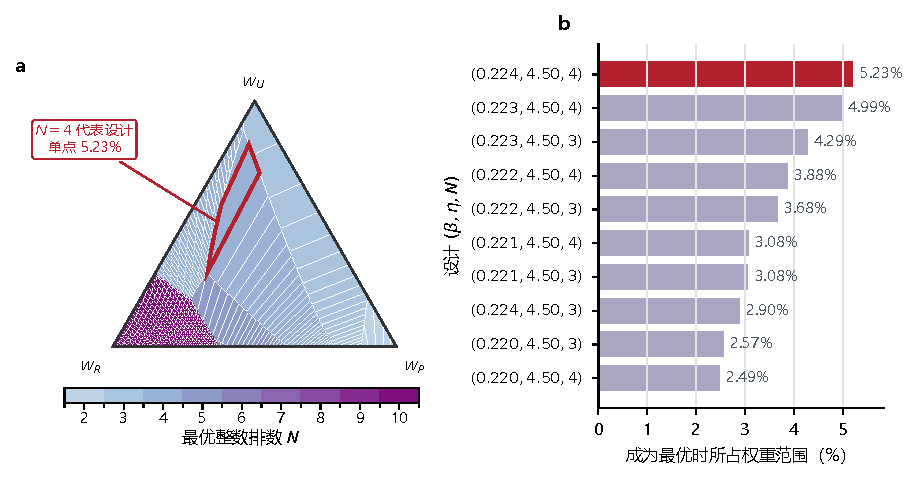
\includegraphics[width=0.90\textwidth]{fig_q4_weight_acceptability.pdf}
\caption{权重三角形中的最优设计分区。（a）按使加权得分最小的整数排数以蓝紫顺序色着色；半透明白线表示同一排数内不同设计的边界，红色轮廓标出区域内选取的代表设计。（b）权重范围最大的 10 个候选方案，代表设计以红色标出。}
\label{fig:q4-weight-acceptability}
\end{figure}

图~\ref{fig:q4-weight-acceptability}(a) 中，不同权重对应的最优排数形成了清晰的分区，其中较大的连续区域主要属于 $N=3$--$4$。图~\ref{fig:q4-weight-acceptability}(b) 中排名靠前的设计也均位于 $\beta\approx0.22$、$\eta=4.5$ 附近。据此，将区域 $\mathcal C$ 作为问题四的推荐参数范围，并以单点权重范围最大的 $(0.224,4.50,4)$ 作为其中的代表方案。

\section{问题五：参数误差与工况变化}
\subsection{相对敏感度}
问题三给出了没有额外权重信息时的推荐设计，问题四则选择了对指标权重相对不敏感的设计。实际加工中，$\beta$ 和 $\eta$ 难免偏离设计值，需要判断小范围尺寸误差是否会明显改变性能。附件只定义了这两个几何比值，没有给出各独立尺寸的制造公差，因而直接考察 $\beta$ 和 $\eta$ 的相对误差。设计点附近的变化用局部导数描述。误差达到几个百分点时，再计算给定范围内可能出现的最大性能变化。

下面比较问题三方案与问题四代表方案。$\beta$、$\eta$ 以及三个指标的数值尺度不同，普通偏导数不宜直接横向比较。保持整数 $N$ 不变，对 $p_k\in\{\beta,\eta\}$ 定义相对敏感度
\begin{equation}
S_{jk}=\left|\frac{p_k}{\hat f_j}\frac{\partial\hat f_j}{\partial p_k}\right|.
\end{equation}
$S_{jk}$ 给出参数相对变化 $1\%$ 时指标的近似百分比变化。问题三方案中，压降对 $\eta$ 和 $\beta$ 的敏感度分别为 0.865 和 0.500。问题四代表方案中相应数值为 0.983 和 0.290。两种方案的热阻对 $\eta$ 的敏感度均约为 0.15，明显高于其对 $\beta$ 的敏感度。两个方案都位于 $\eta=4.5$ 的上边界，所以这里的 $\eta$ 敏感度只衡量 $\eta$ 向参数范围内部减小时的局部变化。变化方向仍由偏导数符号判断，结论不外推至 $\eta>4.5$。

\subsection{假设参数误差下的最大影响}
$\pm1\%$、$\pm3\%$ 和 $\pm5\%$ 是本文设定的相对误差，不是真实制造公差。设置三档误差，用于观察误差范围扩大后性能变化是否仍近似线性。定义
\begin{equation}
\Omega_\delta=\{(\tilde\beta,\tilde\eta):
|\tilde\beta/\beta-1|\leq\delta,|\tilde\eta/\eta-1|\leq\delta\}.
\end{equation}
令 $\mathcal D=[0.10,0.30]\times[3.0,4.5]$ 为预测模型的连续参数范围。保持 $N$ 不变，对指标 $f_j$ 定义最大相对增幅
\begin{equation}
\begin{aligned}
D_j^{\max}(\delta)=
\max_{(\tilde\beta,\tilde\eta)\in\Omega_\delta\cap\mathcal D}
\frac{\hat f_j(\tilde\beta,\tilde\eta,N)-\hat f_j(\beta,\eta,N)}
{\hat f_j(\beta,\eta,N)}\times100\%.
\end{aligned}
\label{eq:worst-case}
\end{equation}
为便于比较两个方案，取三项最大增幅中的最大值作为总体最大增幅：
\begin{equation}
D_{\mathrm{all}}^{\max}(\delta)=
\max_{j\in\{R,P,U\}}D_j^{\max}(\delta).
\label{eq:overall-worst-case}
\end{equation}
计算时，先分别求取三项指标在给定误差范围内的最大增幅，再按式~\eqref{eq:overall-worst-case} 取其中最大者，总体值无需另行优化。各指标先用固定随机种子的差分进化算法计算\cite{StornPrice1997}，再作有界局部优化。两个方案均位于 $\eta=4.5$，误差区间在该处截断。式~\eqref{eq:worst-case} 的结果见表~\ref{tab:q5}。
\begin{table}[H]
\centering
\caption{假设参数误差下各指标的最大相对增幅（\%）}
\label{tab:q5}
\begin{tabular}{lcccccc}
\toprule
& \multicolumn{3}{c}{问题三方案} & \multicolumn{3}{c}{问题四代表方案}\\
\cmidrule(lr){2-4}\cmidrule(lr){5-7}
$\delta$ & $\Rstar$ & $\Pstar$ & $\Ustar$ & $\Rstar$ & $\Pstar$ & $\Ustar$\\
\midrule
$1\%$ & 0.160 & 1.374 & 0.132 & 0.149 & 1.281 & 0.175\\
$3\%$ & 0.420 & 4.182 & 0.326 & 0.386 & 3.898 & 0.444\\
$5\%$ & 0.608 & 7.096 & 0.440 & 0.547 & 6.618 & 0.627\\
\bottomrule
\end{tabular}
\end{table}
两种设计中，压降受几何误差的影响最大。$\delta=1\%,3\%,5\%$ 时，问题三方案的总体最大增幅依次为 1.374\%、4.182\%、7.096\%，问题四代表方案依次为 1.281\%、3.898\%、6.618\%。六种情形的总体最大增幅均由 $\Pstar$ 决定。问题四代表方案的压降和热阻最大增幅略小，温度非均匀性的增幅则较大。
\begin{figure}[!htbp]
\centering
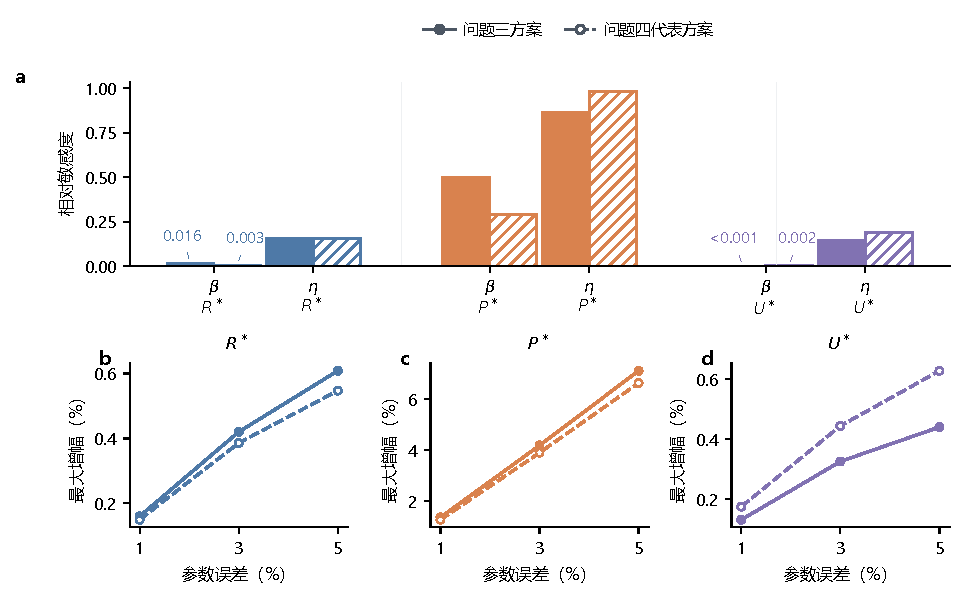
\includegraphics[width=\textwidth]{fig_q5_parameter_error_analysis.pdf}
\caption{两个代表方案的参数误差比较。（a）相对敏感度；（b）--（d）假设误差范围增大时三项指标的最大相对增幅。实线和实心点表示问题三方案，虚线和空心点表示问题四代表方案。}
\label{fig:q5-parameter-error-analysis}
\end{figure}

图~\ref{fig:q5-parameter-error-analysis} 显示，在 $1\%$--$5\%$ 的误差范围内，两种方案各项性能的变化均较平滑，没有出现突变。压降始终是最敏感的性能指标。问题四方案对权重选择相对不敏感，但不能据此认为它对尺寸误差也不敏感。

\subsection{工况变化的尺度分析}
以额定质量流量 $\dot m_0=1.0\,\mathrm{g\,s^{-1}}$ 和芯片发热量 $36\,\mathrm W$ 为基准，式~\eqref{eq:coolant-rise} 给出的平均温升为 $8.61\,\mathrm K$。令 $\lambda_m=\dot m/\dot m_0$，在冷却液物性和带走热量近似不变时，
\begin{equation}
\Delta\bar T_f(\lambda_m)=\frac{8.61}{\lambda_m}\ \mathrm K.
\end{equation}
当 $\lambda_m=0.9,1.0,1.1$ 时，平均温升依次为 9.56 K、8.61 K 和 7.83 K。质量流量降低 10\% 时，平均温升约增加 11.1\%，提高 10\% 时则约降低 9.1\%。增大流量通常还会强化对流换热并提高系统压降，但附件没有变流量样本，无法确定压降增幅及三项无量纲指标的变化量。入口温度主要改变绝对温度水平，热源强度则同时改变固体与冷却液温升，这两项变化都不用于方案重新排序。Sarangi 等（2014）曾研究不确定条件下的歧管式微通道优化\cite{Sarangi2014}。若要比较两个方案在变工况下的性能，还需补充相应工况样本。

\section{模型特点与局限}
\subsection{主要特点}
本文以支路压差和流量为纽带，把歧管内的流量分配、针肋换热和芯片导热联系起来，并据此解释后续数据模型中的性能变化。无针肋样本只用于检验压降尺度关系，有针肋样本则用于建立三次响应面，避免在缺少过渡数据时混合两类结构。

代理模型的检验除五折交叉验证和留一验证外，还分别整体留出中间 $N$ 水平和中央 $(\beta,\eta)$ 参数区域，用于检查模型对未观测排数和局部参数空缺的插值能力。

优化时先在没有明确权重的情况下选择三项性能较为均衡的方案，再改变指标权重，观察优选设计在权重三角形中的分布。为减小网格步长的影响，问题四还将相邻设计合并为推荐区域。问题五随后比较两种代表方案受几何扰动时的性能变化，并估算质量流量改变后的冷却液平均温升。
\subsection{局限}
问题一缺少局部尺寸、损失系数和支路压力，只能用于解释结构参数的作用，不能代替完整 CFD。响应面依据单一工况下的确定性数据建立，工程预测能力仍需实验验证。奇数 $N$ 的插值结果、$\eta>4.5$ 时的变化趋势和变工况响应也需要新增样本支持。问题五设定的误差范围仅供方案比较，不代表真实制造公差。

\section{结论}
各部分对 $\beta$ 和 $\eta$ 的结论基本一致：优选设计的针肋宽度比集中在 $\beta\approx0.22$，歧管深高比在现有样本范围内倾向于取上界 $\eta=4.5$。不同评价准则的差异主要体现在针肋排数 $N$：无明确权重时推荐 $N=6$，而在权重变化下，适用范围较大的设计主要集中在 $N=3$--$4$。
\begin{enumerate}
  \item 在附件范围内，$\eta$ 增大时压降明显下降，$\beta$ 和 $N$ 同时影响换热与阻力。无针肋压降近似满足 $\eta^{-2}$ 关系。加入 $N\beta^2$ 后，简化关系对全部 84 组数据的拟合达到 $R^2=0.9764$。
  \item 三次响应面在五折交叉验证中的三项 RMSE 均不超过 $5.59\times10^{-4}$。留出中央 20 组相邻参数组合后，三项 RMSE 仍不超过 $4.29\times10^{-4}$。
  \item 以最大归一化偏差最小为准，问题三推荐 $\beta\approx0.225$、$\eta=4.50$、$N=6$，其中连续优化值为 $\beta=0.22494$。其 $\Rstar$、$\Pstar$ 和 $\Ustar$ 依次为 0.73433、0.09800 和 0.79019。
  \item 仅依据主网格确定的邻近设计区域为 $0.215\leq\beta\leq0.224$、$\eta=4.5$、$N=3$--4，覆盖 51.66\% 的权重组合。固定边界后，偶数排数和加密网格复算得到的覆盖率分别为 48.38\% 和 49.99\%，$(0.224,4.50,4)$ 可作为代表方案。
  \item 在附件参数范围内考虑不超过 $5\%$ 的 $\beta$ 和 $\eta$ 误差时，两种方案的总体最大增幅分别为 7.10\% 和 6.62\%，均由压降控制。质量流量取额定值的 0.9 倍和 1.1 倍时，冷却液平均温升约为 9.56 K 和 7.83 K。三项无量纲指标在变工况下的变化仍需新增样本验证。
\end{enumerate}

\section*{AI 工具使用声明}
本参赛队在竞赛过程中使用了 ChatGPT 网页端的 \mbox{GPT-5.6 Sol} 模型和 Codex 应用，辅助开展赛题分析与建模讨论、Python 代码编写和调试、数值结果核验、图表修改、参考文献核对以及论文文字和 \LaTeX{} 排版修改。参赛队员对 AI 辅助内容进行了审查、修改和核实，具体使用情况见支撑材料。

\bibliographystyle{gbt7714-numerical}
\setlength{\bibsep}{0.25em}
\bibliography{references}

\clearpage
\section{附录}
\setcounter{subsection}{0}
\renewcommand{\thesubsection}{\Alph{subsection}}
\subsection{三次响应面系数}
式~\eqref{eq:cubic} 采用式~\eqref{eq:encoding} 定义的编码变量。表~\ref{tab:cubic-coefficients} 列出三个指标的全部 20 项系数。将各行系数与首列基函数相乘后求和，即可计算 $\hat R^*$、$\hat P^*$ 和 $\hat U^*$。
\begin{table}[H]
\centering
\caption{三次响应面的拟合系数}
\label{tab:cubic-coefficients}
\scriptsize
\setlength{\tabcolsep}{7pt}
\renewcommand{\arraystretch}{1.04}
\begin{tabular}{crrr}
\toprule
基函数 & $\theta_R$ & $\theta_P$ & $\theta_U$\\
\midrule
$1$             & $ 7.382200533\times10^{-1}$ & $ 1.096298204\times10^{-1}$ & $ 7.891945219\times10^{-1}$\\
$x_3$           & $-5.308693996\times10^{-3}$ & $ 2.126722854\times10^{-2}$ & $ 3.993767977\times10^{-2}$\\
$x_2$           & $ 8.539480117\times10^{-3}$ & $-2.075778929\times10^{-2}$ & $ 7.575959930\times10^{-3}$\\
$x_1$           & $-1.004597109\times10^{-2}$ & $ 1.493687160\times10^{-2}$ & $-1.371825425\times10^{-2}$\\
$x_3^2$         & $ 5.767732653\times10^{-3}$ & $-2.987912245\times10^{-3}$ & $ 8.594963265\times10^{-3}$\\
$x_2x_3$        & $-7.823340000\times10^{-4}$ & $-1.215917143\times10^{-4}$ & $ 4.447044000\times10^{-3}$\\
$x_2^2$         & $-3.930965357\times10^{-3}$ & $ 7.123924286\times10^{-3}$ & $ 1.103021357\times10^{-2}$\\
$x_1x_3$        & $-4.959048182\times10^{-3}$ & $ 1.700184500\times10^{-2}$ & $ 4.854860909\times10^{-3}$\\
$x_1x_2$        & $-1.179002182\times10^{-3}$ & $-3.117163636\times10^{-5}$ & $ 5.431969636\times10^{-3}$\\
$x_1^2$         & $ 1.082530000\times10^{-2}$ & $ 1.211110000\times10^{-2}$ & $ 2.139310000\times10^{-2}$\\
$x_3^3$         & $-6.938458333\times10^{-3}$ & $-6.764166667\times10^{-3}$ & $-2.920550000\times10^{-2}$\\
$x_2x_3^2$      & $ 7.820067857\times10^{-3}$ & $ 8.677821429\times10^{-4}$ & $-1.890921429\times10^{-3}$\\
$x_2^2x_3$      & $ 3.474590625\times10^{-3}$ & $ 1.281656250\times10^{-4}$ & $ 2.896312500\times10^{-3}$\\
$x_2^3$         & $-6.215287500\times10^{-3}$ & $-2.509734375\times10^{-3}$ & $-1.542479063\times10^{-2}$\\
$x_1x_3^2$      & $ 1.056289796\times10^{-3}$ & $-3.178297959\times10^{-3}$ & $ 3.286848980\times10^{-3}$\\
$x_1x_2x_3$     & $-4.794252000\times10^{-3}$ & $-2.551937143\times10^{-4}$ & $-1.690728000\times10^{-3}$\\
$x_1x_2^2$      & $-1.362972857\times10^{-3}$ & $-1.331807143\times10^{-4}$ & $-8.148516429\times10^{-3}$\\
$x_1^2x_3$      & $ 2.554954545\times10^{-3}$ & $ 5.414050000\times10^{-3}$ & $-2.965572727\times10^{-3}$\\
$x_1^2x_2$      & $ 1.395774545\times10^{-3}$ & $-3.556690909\times10^{-4}$ & $ 5.001889091\times10^{-3}$\\
$x_1^3$         & $ 6.139533333\times10^{-3}$ & $ 6.238866667\times10^{-3}$ & $ 1.750653333\times10^{-2}$\\
\bottomrule
\end{tabular}
\end{table}

\subsection{支撑材料与核心源代码}
整理后的数据、复算程序、数值结果和论文图件均保存在项目目录中，各目录的作用及主要文件见表~\ref{tab:supporting-files}。完整运行方法和环境依赖见根目录下的 \path{README.md}，主要复现命令为
\begin{lstlisting}
python scripts/run_analysis.py
python scripts/make_figures.py
python -m pytest -q
\end{lstlisting}
机器可读的响应面系数、Pareto 网格、加密网格检查、权重区域和参数误差结果均保存在 \path{outputs/tables/} 目录。
\begin{table}[H]
\centering
\caption{论文支撑材料及用途}
\label{tab:supporting-files}
\footnotesize
\setlength{\tabcolsep}{4pt}
\renewcommand{\arraystretch}{1.02}
\begin{tabularx}{\textwidth}{>{\raggedright\arraybackslash}p{0.32\textwidth}>{\raggedright\arraybackslash}X}
\toprule
文件或目录 & 内容\\
\midrule
\path{data/processed/attachment2_tidy.csv} & 按样本编号和参数列整理后的附件 2 数据，供人工核对和其他程序直接读取\\
\path{src/mmc_model/} & 数据校验、问题一计算、三次响应面、模型验证、多目标优化、权重范围和参数误差分析函数\\
\path{scripts/run_analysis.py} & 读取附件 2，依次完成数据核对、模型拟合与验证、问题三至问题五计算，并更新全部机器可读结果\\
\path{scripts/make_figures.py} & 读取计算结果，生成问题一数据检验、响应面验证、多目标优化、权重分析和参数误差分析图\\
\path{outputs/results.json} & 保存主要模型指标、推荐设计、目标值、优化器设置、权重汇总值和稳定性检查结果\\
\path{outputs/tables/} & 保存问题一至问题五的 17 个 CSV 结果表，包括响应面系数、4293 个 Pareto 点、中央 20 组相邻参数的留出结果、邻近设计区域、总体最大增幅和流量情景结果\\
\path{outputs/figures/} & 保存 PowerPoint 绘图源文件及其导出的 5 个示意图，以及 Python 生成的 6 组数据图，数据图均提供 PDF、SVG、PNG 和 TIFF 四种格式\\
\path{tests/test_models.py} & 数据结构、能量与流量守恒、响应面精度、中央 20 组相邻参数留出、Pareto 筛选、邻近设计区域和总体最大增幅的回归测试\\
\path{README.md}、\path{pyproject.toml} & 项目结构、环境依赖、复现命令和 Python 工程配置\\
\bottomrule
\end{tabularx}
\end{table}

\subsubsection{核心源代码}
为便于核查论文中的主要计算过程，本节全文列出直接实现数据校验、问题一计算、响应面拟合与预测验证、多目标优化及误差分析的五个模块。主运行脚本负责组织计算并写出结果，绘图脚本只负责生成图件，测试文件用于回归检查，各 Python 文件的作用见表~\ref{tab:code-files}。

\begin{table}[H]
\centering
\caption{Python 代码文件说明}
\label{tab:code-files}
\footnotesize
\setlength{\tabcolsep}{4pt}
\renewcommand{\arraystretch}{1.05}
\begin{tabularx}{\textwidth}{>{\raggedright\arraybackslash}p{0.34\textwidth}>{\raggedright\arraybackslash}X}
\toprule
文件 & 主要作用\\
\midrule
\path{src/mmc_model/__init__.py} & 定义模型包的公开接口，导出数据读取函数和三次响应面类\\
\path{src/mmc_model/data.py} & 定位并读取附件 2，检查样本编号、参数组合和响应值，并区分无针肋与有针肋样本\\
\path{src/mmc_model/q1.py} & 计算歧管流量守恒、冷却液能量平衡、压降简化关系及平衡试验的参数影响\\
\path{src/mmc_model/rsm.py} & 完成变量编码、三次响应面的拟合和预测，并计算响应梯度与设计矩阵条件数\\
\path{src/mmc_model/validation.py} & 实现五折交叉验证、留一验证、整组留出 $N=4,6,8$、整体留出中央 20 组相邻参数及高斯过程基准模型\\
\path{src/mmc_model/optimization.py} & 实现目标极值搜索、Pareto 筛选、Chebyshev 折中、权重区域裁剪及单项和总体最大增幅计算\\
\path{scripts/run_analysis.py} & 串联五问计算，统一保存 JSON 和 CSV 结果，是项目的主运行入口\\
\path{scripts/make_figures.py} & 读取计算结果并生成论文中的 6 组数据图，不参与模型参数估计\\
\path{tests/test_models.py} & 检查数据结构、守恒关系、预测精度、Pareto 筛选、权重区域及稳定性结果\\
\bottomrule
\end{tabularx}
\end{table}

\lstinputlisting[
  style=pythonappendix,
  caption={数据读取与完整性校验（\texttt{data.py}）},
  label={lst:data}
]{../../../src/mmc_model/data.py}

\lstinputlisting[
  style=pythonappendix,
  caption={问题一的守恒关系、压降拟合与参数影响计算（\texttt{q1.py}）},
  label={lst:q1}
]{../../../src/mmc_model/q1.py}

\lstinputlisting[
  style=pythonappendix,
  caption={三次响应面的拟合、预测与梯度计算（\texttt{rsm.py}）},
  label={lst:rsm}
]{../../../src/mmc_model/rsm.py}

\lstinputlisting[
  style=pythonappendix,
  caption={响应面验证与基准模型比较（\texttt{validation.py}）},
  label={lst:validation}
]{../../../src/mmc_model/validation.py}

\lstinputlisting[
  style=pythonappendix,
  caption={多目标优化、权重范围与参数误差分析（\texttt{optimization.py}）},
  label={lst:optimization}
]{../../../src/mmc_model/optimization.py}
\end{document}
